\documentclass[9pt,a4paper,]{extarticle}

\usepackage{f1000_styles}

\usepackage[pdfborder={0 0 0}]{hyperref}

\usepackage[numbers]{natbib}
\bibliographystyle{unsrtnat}


%% maxwidth is the original width if it is less than linewidth
%% otherwise use linewidth (to make sure the graphics do not exceed the margin)
\makeatletter
\def\maxwidth{ %
  \ifdim\Gin@nat@width>\linewidth
    \linewidth
  \else
    \Gin@nat@width
  \fi
}
\makeatother

\usepackage{color}
\usepackage{fancyvrb}
\newcommand{\VerbBar}{|}
\newcommand{\VERB}{\Verb[commandchars=\\\{\}]}
\DefineVerbatimEnvironment{Highlighting}{Verbatim}{commandchars=\\\{\}}
% Add ',fontsize=\small' for more characters per line
\usepackage{framed}
\definecolor{shadecolor}{RGB}{248,248,248}
\newenvironment{Shaded}{\begin{snugshade}}{\end{snugshade}}
\newcommand{\AlertTok}[1]{\textcolor[rgb]{0.94,0.16,0.16}{#1}}
\newcommand{\AnnotationTok}[1]{\textcolor[rgb]{0.56,0.35,0.01}{\textbf{\textit{#1}}}}
\newcommand{\AttributeTok}[1]{\textcolor[rgb]{0.13,0.29,0.53}{#1}}
\newcommand{\BaseNTok}[1]{\textcolor[rgb]{0.00,0.00,0.81}{#1}}
\newcommand{\BuiltInTok}[1]{#1}
\newcommand{\CharTok}[1]{\textcolor[rgb]{0.31,0.60,0.02}{#1}}
\newcommand{\CommentTok}[1]{\textcolor[rgb]{0.56,0.35,0.01}{\textit{#1}}}
\newcommand{\CommentVarTok}[1]{\textcolor[rgb]{0.56,0.35,0.01}{\textbf{\textit{#1}}}}
\newcommand{\ConstantTok}[1]{\textcolor[rgb]{0.56,0.35,0.01}{#1}}
\newcommand{\ControlFlowTok}[1]{\textcolor[rgb]{0.13,0.29,0.53}{\textbf{#1}}}
\newcommand{\DataTypeTok}[1]{\textcolor[rgb]{0.13,0.29,0.53}{#1}}
\newcommand{\DecValTok}[1]{\textcolor[rgb]{0.00,0.00,0.81}{#1}}
\newcommand{\DocumentationTok}[1]{\textcolor[rgb]{0.56,0.35,0.01}{\textbf{\textit{#1}}}}
\newcommand{\ErrorTok}[1]{\textcolor[rgb]{0.64,0.00,0.00}{\textbf{#1}}}
\newcommand{\ExtensionTok}[1]{#1}
\newcommand{\FloatTok}[1]{\textcolor[rgb]{0.00,0.00,0.81}{#1}}
\newcommand{\FunctionTok}[1]{\textcolor[rgb]{0.13,0.29,0.53}{\textbf{#1}}}
\newcommand{\ImportTok}[1]{#1}
\newcommand{\InformationTok}[1]{\textcolor[rgb]{0.56,0.35,0.01}{\textbf{\textit{#1}}}}
\newcommand{\KeywordTok}[1]{\textcolor[rgb]{0.13,0.29,0.53}{\textbf{#1}}}
\newcommand{\NormalTok}[1]{#1}
\newcommand{\OperatorTok}[1]{\textcolor[rgb]{0.81,0.36,0.00}{\textbf{#1}}}
\newcommand{\OtherTok}[1]{\textcolor[rgb]{0.56,0.35,0.01}{#1}}
\newcommand{\PreprocessorTok}[1]{\textcolor[rgb]{0.56,0.35,0.01}{\textit{#1}}}
\newcommand{\RegionMarkerTok}[1]{#1}
\newcommand{\SpecialCharTok}[1]{\textcolor[rgb]{0.81,0.36,0.00}{\textbf{#1}}}
\newcommand{\SpecialStringTok}[1]{\textcolor[rgb]{0.31,0.60,0.02}{#1}}
\newcommand{\StringTok}[1]{\textcolor[rgb]{0.31,0.60,0.02}{#1}}
\newcommand{\VariableTok}[1]{\textcolor[rgb]{0.00,0.00,0.00}{#1}}
\newcommand{\VerbatimStringTok}[1]{\textcolor[rgb]{0.31,0.60,0.02}{#1}}
\newcommand{\WarningTok}[1]{\textcolor[rgb]{0.56,0.35,0.01}{\textbf{\textit{#1}}}}

% disable code chunks background
%\renewenvironment{Shaded}{}{}

% disable section numbers
\setcounter{secnumdepth}{0}

%% added by MLS, this is not in the F1000 style by default %%

\hypersetup{unicode=true,
            pdftitle={sSNAPPY: an R/Bioconductor package for single-sample directional pathway perturbation analysis},
            pdfkeywords={RNA-seq, pathway enrichment, R package, topology, KEGG, Reactome, scRNA-seq},
            pdfborder={0 0 0},
            breaklinks=true}

%% End added by MLS %%

\setlength{\parindent}{0pt}
\setlength{\parskip}{6pt plus 2pt minus 1pt}


\usepackage{endfloat}
\usepackage{booktabs}
\usepackage{longtable}
\usepackage{booktabs}
\usepackage{longtable}
\usepackage{array}
\usepackage{multirow}
\usepackage{wrapfig}
\usepackage{float}
\usepackage{colortbl}
\usepackage{pdflscape}
\usepackage{tabu}
\usepackage{threeparttable}
\usepackage{threeparttablex}
\usepackage[normalem]{ulem}
\usepackage{makecell}
\usepackage{xcolor}

\begin{document}
\pagestyle{front}

\title{sSNAPPY: an R/Bioconductor package for single-sample directional pathway perturbation analysis}

\author[1]{Wenjun Liu\thanks{\ttfamily Corresponding Author wenjun.liu@adelaide.edu.au}}
\author[2,3]{Ville-Petteri Mäkinen}
\author[1]{Wayne D. Tilley}
\author[1,4,5]{Stephen M. Pederson}
\affil[1]{Dame Roma Mitchell Cancer Research Laboratories, Adelaide Medical School, Faculty of Health and Medical Sciences, University of Adelaide, Adelaide, Australia}
\affil[2]{Computational Medicine, Faculty of Medicine, University of Oulu, Oulu, Finland}
\affil[3]{Center for Life Course Health Research, Faculty of Medicine, University of Oulu, Oulu, Finland}
\affil[4]{Black Ochre Data Laboratories, Telethon Kids Institute, Adelaide, Australia}
\affil[5]{John Curtin School of Medical Research, Australian National University, Canberra, Australia}

\maketitle
\thispagestyle{front}

\begin{abstract}
A common outcome of analysing RNA-Seq data is the detection of biological pathways with significantly altered activity between the conditions under investigation. Whilst many strategies test for over-representation within pre-defined gene-sets for genes showing changed expression, these analyses typically do not account for gene-gene interactions encoded by pathway topologies, and are not able to directly predict the directional change of pathway activity. To address these issues, we have developed a single-sample pathway perturbation analysis method \href{https://bioconductor.org/packages/sSNAPPY}{\emph{sSNAPPY}}, now available as an R/Bioconductor package, which leverages pathway topology information to compute pathway perturbation scores, and predicts the direction of change across a set of pathways. Here, we demonstrate the use of \emph{sSNAPPY} by applying the method to public scRNA-seq data, derived from ovarian cancer patient tissues collected before and after chemotherapy. Not only were we able to predict the directions of significant perturbations of pathways discussed in the original study, but \emph{sSNAPPY} was also able to detect significant changes of other biological processes, yielding far greater insight into the response to treatment. \emph{sSNAPPY} represents a novel pathway analysis strategy that takes into consideration of pathway topology to predict impacted biology pathways, both within related samples and across treatment groups. In addition to not relying on the detection of differentially expressed genes, the method and associated R package offer important flexibility and provide powerful visualisation tools.
\end{abstract}

\section*{Keywords}
RNA-seq, pathway enrichment, R package, topology, KEGG, Reactome, scRNA-seq


\clearpage
\pagestyle{main}

\textbf{R version}: R version 4.3.0 (2023-04-21)

\textbf{Bioconductor version}: 3.17

\textbf{Package}: 1.5.4

\hypertarget{introduction}{%
\section{Introduction}\label{introduction}}

Using pathway enrichment analysis to gain biological insights from gene expression data is a pivotal step in the analysis and interpretation of RNA-seq data, for which numerous methods have been developed (reviewed in \citep{Maleki2020-ur, Mubeen2022-eq}).
Many existing methods tend to view pathways simply as a collection of gene names, as seen in those relying on the detection of differentially expressed genes and applying over-representation analysis (ORA) strategies, and those scoring all genes using functional class scoring (FCS), such as in Gene Set Enrichment Analysis (GSEA)\citep{Subramanian2005-lx}, arguably the most widely-used approach.
However, databases such as the Kyoto Encyclopaedia of Genes and Genomes (KEGG)\citep{OgataKEGGKyotoEncyclopediaa} and WikiPathways\citep{Martens2021} capture not only which genes are implicated in a certain biological process but also their interactions, activating or inhibitory roles, and their relative importance within the pathway, all of which are overlooked in ORA- and FCS-based approaches.

To fully utilise that additional information, the latest generation of pathway analysis approaches include many which are topology-based such as SPIA\citep{Tarca2009}, DEGraph\citep{Jacob2012}, NetGSA\citep{Ma2016} and PRS\citep{Ibrahim2012}, as well as others which explicitly model inter-gene correlations\citep{Wu2012}.
Despite differences in the null hypotheses tested across these approaches, overall, they have demonstrated enhanced sensitivity and specificity due to their abilities to take gene-gene interconnections into account\citep{Nguyen2019-va, Ma2019}.
Nevertheless, most topology-based methods focus only on comparing activities of pathways between two treatment groups and cannot be used to score individual samples (Figure \ref{fig:Figure1}).
However, in heterogenous data where more than one factor may be influencing observations\citep{Hanzelmann2013}, incorporating scoring within paired samples may be desirable and may be able to reveal more nuanced insights.
To address this gap, we present a Single-Sample directioNAl Pathway Perturbation analYsis methodology called \href{https://bioconductor.org/packages/sSNAPPY}{\emph{sSNAPPY}}, available as an R/Bioconductor package.
This article defines how \emph{sSNAPPY} computes changes in gene expression within paired samples, and propagates this through gene-set topologies to predict the perturbation in pathway activities within paired samples, before providing summarised results across an entire dataset (Figure \ref{fig:Figure1}).
The practical usage of the \emph{sSNAPPY} R/Bioconductor package is illustrated through the analysis of a public scRNA-seq dataset using the pseudo-bulk strategy.

\begin{figure}

{\centering 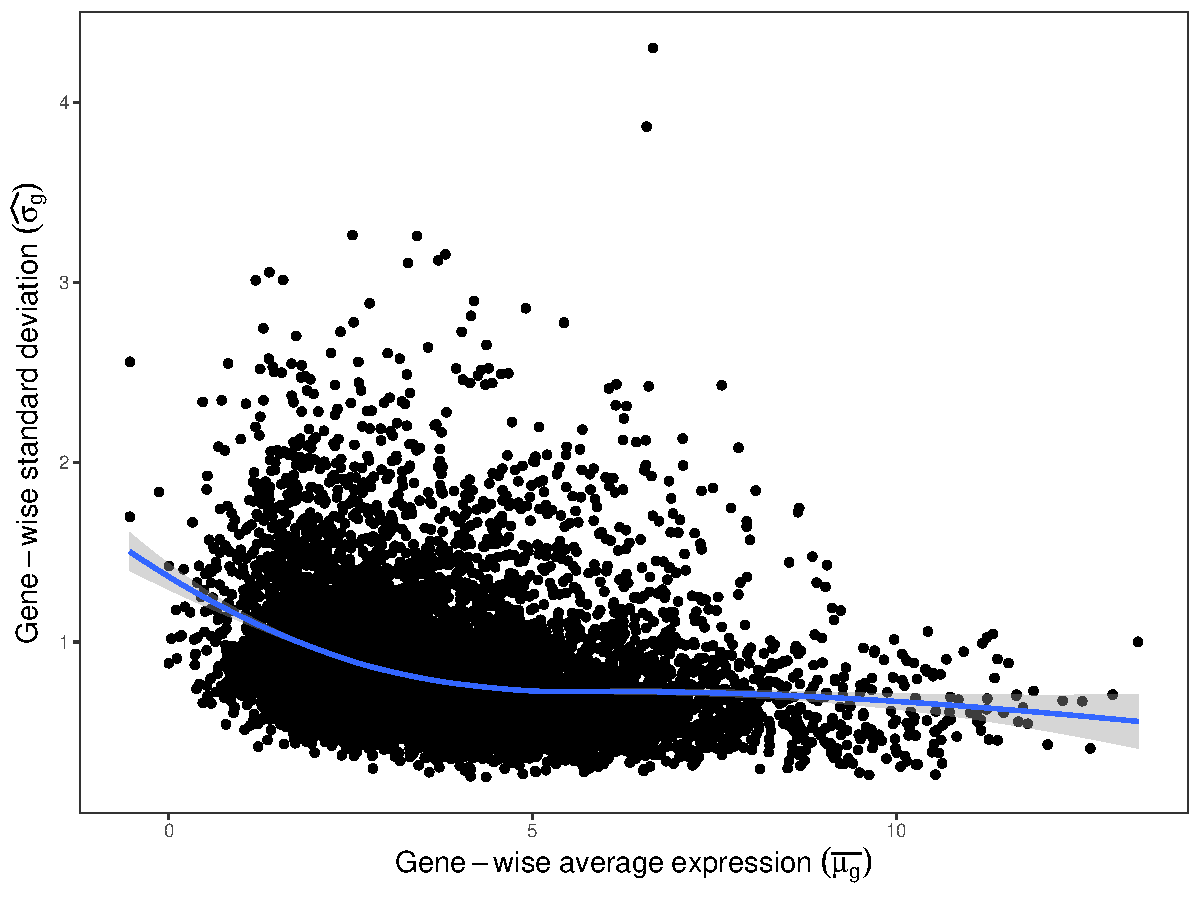
\includegraphics[width=1\linewidth]{sSNAPPY_paper_files/figure-latex/Figure1} 

}

\caption{Schematic illustration of the differences betweeen conventional pathway analysis methods and sSNAPPY. Instead of being limited to treatment-level analyses, \textit{sSNAPPY} allows the detection of pathway perturbation in individual samples by using sample-specific estimates of fold-change instead of experiment-wide estimates. (Created with BioRender.com).}\label{fig:Figure1}
\end{figure}

\hypertarget{methods}{%
\section{Methods}\label{methods}}

\hypertarget{implementation}{%
\subsection{Implementation}\label{implementation}}

\emph{sSNAPPY} is an R package that has been reviewed and published on the open-source bioinformatics software platform \href{https://bioconductor.org/packages/release/bioc/html/*sSNAPPY*.html}{Bioconductor} with all source code available via GitHub.
The methodology itself is topology-based, designed to compute directional, single-sample, pathway perturbation scores for gene expression datasets with a matched-pair, or nested design (eg. samples collected before and after treatment).
This allows for the detection of pathway perturbations within all samples from a treatment group, but also within individual samples.
The only data required to run \emph{sSNAPPY}, is a log-transformed expression matrix (e.g.~logCPM) with matching sample metadata describing treatment groups and the nested structure.
It is assumed that all pre-processing has been performed beforehand, such as the exclusion of low-signal genes or normalisation to minimise technical artefacts like GC-bias.

The first step performed by \emph{sSNAPPY}, is to estimate sample-specific log fold-change (\(\delta_{ghi} = \mu_{ghi} - \mu_{g0i}\)) across all genes \(g\) for each treatment \(h\) within each set of nested replicates \(i\), by subtracting expression estimates for the baseline samples \(\mu_{g0i}\) from those in the treatment group \(h\).
Each set of nested replicates may be drawn from treated or control samples within cell-line passages, or from treatments applied to the same donor tissue.
It should also be noted that \emph{sSNAPPY} is applicable to any number of treatment/condition levels and sample numbers within each treatment group are not required to be balanced.

It is well known that in RNA-seq data, genes with lower expression tend to have greater variability in signal and more broadly spread estimates of change\citep{Law2014}.
As such, we utilise a gene-level weighting strategy to down-weight fold-change estimates for low-abundance genes prior to passing these estimates to sSNAPPY.
Gene-level weights \(w_g\) are obtained in a treatment-agnostic manner by fitting a loess curve through the relationship between observed gene-level variance (\(\sigma^2_g\)) and average signal (\(\bar\mu_{g}\))(Figure \ref{fig:Figure2}), and taking the inverse of the loess-predicted variance as the weight \(w_g = a / f(\bar\mu_{g})\), where \(f(\bar\mu_{g})\) is the predicted value from the loess curve and the constant \(a\) ensures \(\sum w_g = 1\).
We then use these weighted estimates of log fold-change (\(\delta_{ghi}^* = w_g\delta_{ghi}\)) in the calculation of all subsequent pathway perturbation scores.

\begin{figure}

{\centering 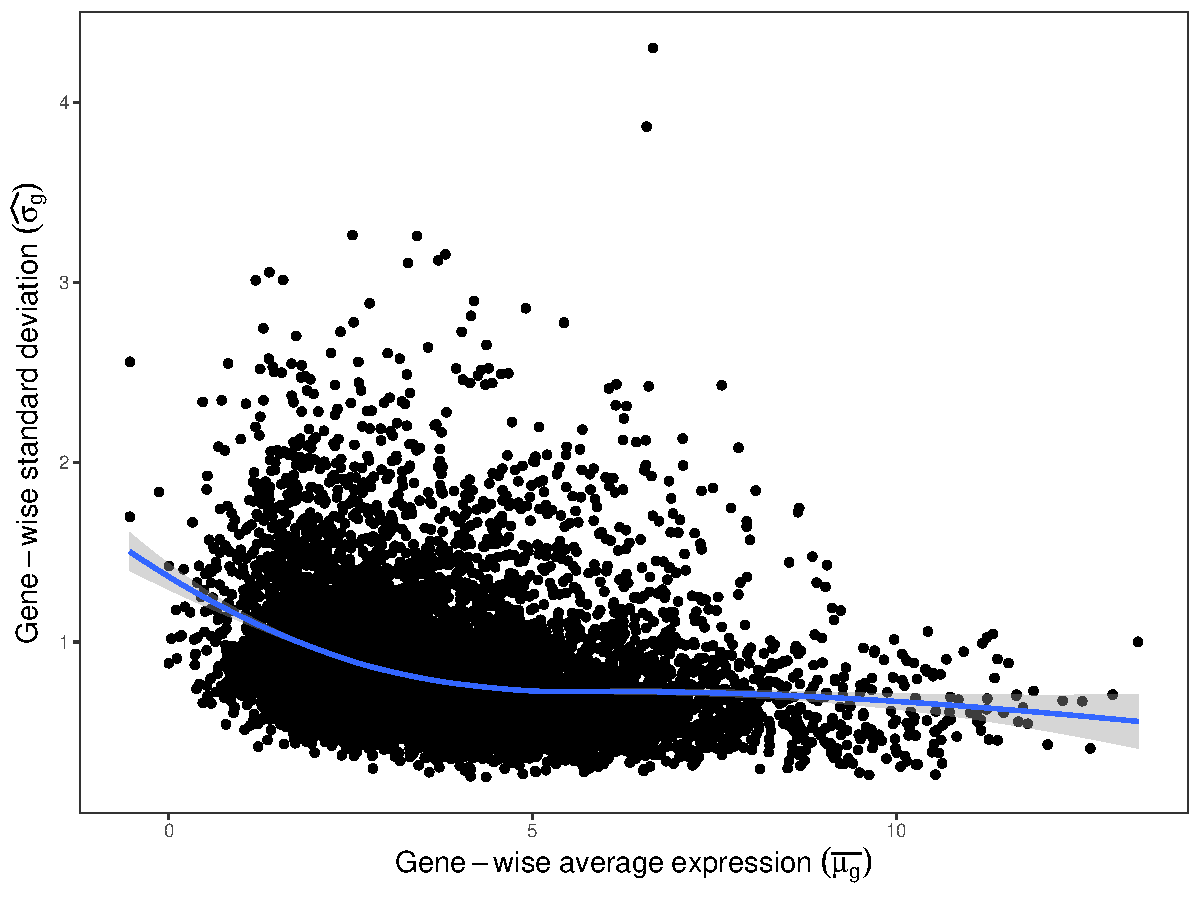
\includegraphics[width=1\linewidth]{sSNAPPY_paper_files/figure-latex/Figure2} 

}

\caption{Gene-wise standard deviations are plotted against the mean logCPM values with mean-variance trend modelled by a loess fit. Whilst standard deviations are shown here for the purposes of visualisation, gene-level weights are calculated using variances at this stage of the sSNAPPY algorithm.}\label{fig:Figure2}
\end{figure}

\emph{sSNAPPY} extends the topology-based scoring algorithm initially proposed in SPIA\citep{Tarca2009} which propagates fold-change estimates from genes considered as differentially expressed through pathway topologies, to compute a perturbation score for each pathway.
In contrast to SPIA, \emph{sSNAPPY} uses fold-change estimates from all detected genes.
By modifying the algorithm to incorporate single-sample, weighted estimates of fold-change, we are able to numerically represent changes in a pathway within a given sample, and subsequently model these across all samples within a treatment group.
Thus, we define the single-sample perturbation score (\(S_{hip}\)) for a given pathway \(p\) and treatment \(h\) for a set of nested samples \(i\):

\[
\begin{aligned}
S_{hip} = \sum_{g \in G_p} \lbrack S_{ghip} - \delta_{ghi}^*\rbrack \text{, where} \\
S_{ghip} = \delta_{ghi}^* + \sum_{g' \in U_{gp}} \beta_{gg'p} \frac{S_{g'hip}}{N_{g'p}} 
\end{aligned}
\]
where:

\begin{itemize}
\item
  \(G_p\) represents the set of genes in pathway \(p\), such that \(g \in G_p\)
\item
  \(S_{ghip}\) is the gene-, treatment- and sample-specific perturbation score for pathway \(p\)
\item
  \(\delta_{ghi}^* = w_g\delta_{ghi}\) is the weighted log fold-change of gene \(g\) as described above
\item
  \(U_{gp}\) is the subset of \(G_p\) containing only the genes directly upstream of gene \(g\)
\item
  \(\beta_{gg'p}\) is the pair-wise gene-gene interactions\citep{Tarca2009} encoded by the topology matrix for genes \(g\) and \(g'\)
\item
  \(N_{gp}\) is the number of downstream genes from any gene \(g\)
\item
  \(S_{hip}\) is the accumulated pathway perturbation score for pathway \(p\) in treatment \(h\) within sample \(i\)
\end{itemize}

To scale single-sample pathway perturbation scores (\(S_{hip}\)) so they are comparable across pathways, and to test for significance of individual scores, null distributions of perturbation scores for each pathway are generated through a sample permutation strategy, which retains any existing correlation structures between genes within a pathway.
During permutation, all sample labels are randomly shuffled and permuted pseudo-pairs formed from the re-shuffled labels.
Single-sample fold-changes are then calculated for each pseudo-pair of permuted samples while the rest of the scoring algorithm remains unchanged.
The median and median absolute deviation (MAD) are calculated from the set of permuted perturbation scores within each pathway, and used to normalise the raw perturbation scores to robust \(Z\)-scores.
All possible permuted pseudo-pairs are sampled unless otherwise specified, such that in an experiment with \(I\) total samples, the maximum number of unique permuted pairs is \({}^IP_2 = \frac{{I!}}{{(I-2)!}} = I \times (I-1)\).
Permutation p-values for individual scores, indicating the approximate significance of pathway perturbation at the single-sample level, are also derived by assessing the proportion of permuted scores with absolute values as extreme, or more extreme, than the absolute value of test perturbation within each pathway\citep{Theo2009}.
Since the smallest achievable permutation p-value is 1/\(NP\), where \(NP\) is the number of permuted pairs, accurate estimation of small p-value requires a large number of permutation that is only feasible in data with large sample size.
As a guideline, GSEA recommends a minimum of 7 samples in each treatment group for utilizing their phenotype permutation approach\citep{GSEAUserGuide}.

Apart from assessing whether a pathway's activity changed significantly within an individual sample, users may also be interested in detecting changes across all samples within a treatment, which can be performed by modelling scores using regression models, and incorporating Smyth's moderated \(t\)-statistic\citep{Smyth_2004} as implemented in \emph{limma}\citep{limma_2015}.
The single-sample nature of \emph{sSNAPPY}'s pathway perturbation scores is particularly helpful for datasets with complex experimental designs or known confounding factors as these can also be incorporated into the final regression models.

The Bioconductor package graphite\citep{Sales2012} provides functions that can be used to retrieve pathway topologies from a database and convert topology information to adjacency matrices.
In order to streamline this process we have implemented a convenience function, where users only need to provide the name of the desired database and species to retrieve all topology information in the format required by the scoring algorithm with the correct type of gene identifiers (ie. Entrez ID).

\hypertarget{operation}{%
\subsection{Operation}\label{operation}}

The package has been tested on all operating systems, requiring R \textgreater{} 4.3.0, and can be installed using BiocManager as follows.

\begin{Shaded}
\begin{Highlighting}[]
\ControlFlowTok{if}\NormalTok{ (}\SpecialCharTok{!}\FunctionTok{requireNamespace}\NormalTok{(}\StringTok{"BiocManager"}\NormalTok{, }\AttributeTok{quietly =} \ConstantTok{TRUE}\NormalTok{))}
  \FunctionTok{install.packages}\NormalTok{(}\StringTok{"BiocManager"}\NormalTok{)}
\NormalTok{BiocManager}\SpecialCharTok{::}\FunctionTok{install}\NormalTok{(}\StringTok{"sSNAPPY"}\NormalTok{)}
\end{Highlighting}
\end{Shaded}

\hypertarget{use-cases}{%
\section{Use Cases}\label{use-cases}}

\hypertarget{data}{%
\subsection{Data}\label{data}}

To demonstrate the application of \emph{sSNAPPY}, we used pre-processed counts from a publicly available scRNA-seq dataset, retrieved from Gene Expression Omnibus (GEO) with accession code GSE165897.
This dataset consists of 11 high-grade serous ovarian cancer (HGSOC) patients samples taken before and after chemotherapy\citep{Zhang2022}.
\emph{sSNAPPY} was used to re-analyse data from the epithelial cells as they were the primary focus of the original study.
Since \emph{sSNAPPY} was designed primarily for bulk RNA-seq data, and as such, counts from epithelial cells within the same samples were first summed into pseudo-bulk profiles, giving rise to a total of 22 samples.
We considered a gene detectable if we observed \textgreater1.5 counts per million in \textgreater11 samples out of 22, ideally representing all samples from a complete treatment group.
11,101 (33.8\%) of the 32,847 annotated genes passed this selection criteria and were included for downstream analyses.
Conditional quantile normalisation\citep{Hansen2012} was then applied to mitigate potential biases introduced by gene length and GC content.
The normalised logCPM matrix of the processed dataset and sample metadata can be downloaded from \href{https://github.com/Wenjun-Liu/F1000_sSNAPPY_manuscript/tree/master/data}{here}.

The following packages are required for this workflow

\begin{Shaded}
\begin{Highlighting}[]
\FunctionTok{library}\NormalTok{(sSNAPPY)}
\FunctionTok{library}\NormalTok{(tidyverse)}
\FunctionTok{library}\NormalTok{(magrittr)}
\FunctionTok{library}\NormalTok{(ggplot2)}
\FunctionTok{library}\NormalTok{(patchwork)}
\FunctionTok{library}\NormalTok{(kableExtra)}
\FunctionTok{library}\NormalTok{(AnnotationHub) }
\FunctionTok{library}\NormalTok{(edgeR)}
\FunctionTok{library}\NormalTok{(patchwork)}
\FunctionTok{library}\NormalTok{(colorspace)}
\end{Highlighting}
\end{Shaded}

To begin running the \emph{sSNAPPY} workflow, we first load our expression matrix and define our sample-level metadata.
Importantly, the row names of the expression matrix must be specified as EntrezGene IDs, for compatibility with pathway databases.
Genes without EntrezGene IDs were excluded during pre-processing, leaving 10,098 genes in the example expression matrix.
The treatment column within our metadata is expected to be a factor, with the reference level interpreted as the control treatment.

\begin{Shaded}
\begin{Highlighting}[]
\NormalTok{logCPM }\OtherTok{\textless{}{-}} \FunctionTok{read\_tsv}\NormalTok{(here}\SpecialCharTok{::}\FunctionTok{here}\NormalTok{(}\StringTok{"data/logCPM.tsv"}\NormalTok{)) }\SpecialCharTok{\%\textgreater{}\%}
    \FunctionTok{column\_to\_rownames}\NormalTok{(}\StringTok{"entrezid"}\NormalTok{)}
\NormalTok{sample\_meta }\OtherTok{\textless{}{-}} \FunctionTok{read\_tsv}\NormalTok{(here}\SpecialCharTok{::}\FunctionTok{here}\NormalTok{(}\StringTok{"data/sample\_meta.tsv"}\NormalTok{), }\AttributeTok{col\_types =} \StringTok{"cfccncnc"}\NormalTok{)}
\FunctionTok{head}\NormalTok{(sample\_meta)}
\end{Highlighting}
\end{Shaded}

\begin{verbatim}
## # A tibble: 6 x 8
##   sample        treatment patient_id anatomical_location   Age Stage   PFI CRS  
##   <chr>         <fct>     <chr>      <chr>               <dbl> <chr> <dbl> <chr>
## 1 EOC372_treat~ treatmen~ EOC372     Peritoneum             68 IIIC    460 1    
## 2 EOC372_post-~ post-NACT EOC372     Peritoneum             68 IIIC    460 1    
## 3 EOC443_post-~ post-NACT EOC443     Omentum                54 IVA     177 3    
## 4 EOC443_treat~ treatmen~ EOC443     Omentum                54 IVA     177 3    
## 5 EOC540_treat~ treatmen~ EOC540     Omentum                62 IIIC    126 2    
## 6 EOC540_post-~ post-NACT EOC540     Omentum                62 IIIC    126 2
\end{verbatim}

\hypertarget{retrieval-of-pathway-topology}{%
\subsection{Retrieval of Pathway Topology}\label{retrieval-of-pathway-topology}}

Next, pathway topology information needs to be retrieved from a chosen database, and this is the only step requiring internet access.
Using the Reactome database\citep{reactome2021} as an example, the retrieved topology information will be stored as a list where each element corresponds to a pathway and the numbers in the matrices encode gene-gene interactions.

\begin{Shaded}
\begin{Highlighting}[]
\NormalTok{gsTopology }\OtherTok{\textless{}{-}} \FunctionTok{retrieve\_topology}\NormalTok{(}\AttributeTok{database =} \StringTok{"reactome"}\NormalTok{, }\AttributeTok{species =} \StringTok{"hsapiens"}\NormalTok{)}
\end{Highlighting}
\end{Shaded}

In addition to downloading topology matrices for all pathways, it is also possible to provide a restricted set of keywords for a targeted analysis.
For example, passing the argument \texttt{keyword\ =\ c("metabolism",\ "estrogen")} would only return the subset of pathways which match either of these keywords.
Multiple databases are also able to be searched by passing a vector of database names to the \texttt{database} argument.

\hypertarget{score-single-sample-pathway-perturbation}{%
\subsection{Score Single-Sample Pathway Perturbation}\label{score-single-sample-pathway-perturbation}}

To compute the single-sample fold-changes (i.e.~logFC) required for the set of perturbation scores, samples must be `matched pairs' or nested, as would be found when analysing biopsies pre- vs post-treatment, or untreated vs treated cell lines nested by passage.
The factor defining the nested structure is passed to the \texttt{weight\_ss\_fc()} function through the \texttt{groupBy} parameter.
In our example dataset, pre- and post-treatment samples are matched by the ``patient\_id'' column.

\begin{Shaded}
\begin{Highlighting}[]
\NormalTok{weightedFC }\OtherTok{\textless{}{-}} \FunctionTok{weight\_ss\_fc}\NormalTok{(}
  \FunctionTok{as.matrix}\NormalTok{(logCPM), }\AttributeTok{metadata =}\NormalTok{ sample\_meta,}
  \AttributeTok{sampleColumn =} \StringTok{"sample"}\NormalTok{, }\AttributeTok{groupBy =} \StringTok{"patient\_id"}\NormalTok{, }\AttributeTok{treatColumn =} \StringTok{"treatment"}
\NormalTok{)}
\FunctionTok{glimpse}\NormalTok{(weightedFC)}
\end{Highlighting}
\end{Shaded}

The output of \texttt{weight\_ss\_fc()} is a \texttt{list} where one element is a matrix of weighted single-sample fold-changes (\(\delta_{ghi}^*\)), with rows corresponding to genes and columns to samples, and the other element is the vector of gene-wise weights (\(w_g\)) used to calculate the weighted log fold-change (\(\delta_{ghi}^*\)), as described above.
By default, the string \texttt{ENTREZID:} is added to all row names of the \(\delta_{ghi}^*\) matrix to be compatible with the format Reactome pathway topologies are retrieved in.

The matrix of \(\delta_{ghi}^*\) values are then passed to pathway topologies to compute gene-wise perturbation scores for all genes within a pathway, before being summed into a single score for each pathway.
\texttt{raw\_gene\_pert()} returns a list, with each element containing the gene-level perturbation scores for a given pathway, with each matrix able to be used during downstream analysis to identify which genes play the most significant roles in each pathway, as demonstrated in later sections.
Pathway-level perturbation scores (\(S_{hip}\)) are then returned as a data.frame containing sample and gene-set names after calling \texttt{pathway\_pert()}.
Pathways with zero perturbation scores across all genes and samples are dropped at this step.

\begin{Shaded}
\begin{Highlighting}[]
\NormalTok{genePertScore }\OtherTok{\textless{}{-}} \FunctionTok{raw\_gene\_pert}\NormalTok{(weightedFC}\SpecialCharTok{$}\NormalTok{weighted\_logFC, gsTopology)}
\NormalTok{ssPertScore }\OtherTok{\textless{}{-}} \FunctionTok{pathway\_pert}\NormalTok{(genePertScore, weightedFC}\SpecialCharTok{$}\NormalTok{weighted\_logFC)}
\FunctionTok{head}\NormalTok{(ssPertScore)}
\end{Highlighting}
\end{Shaded}

\begin{verbatim}
##             sample         score                          gs_name
## 1 EOC372_post-NACT -2.292688e-04 reactome.Interleukin-6 signaling
## 2 EOC443_post-NACT -2.447003e-04 reactome.Interleukin-6 signaling
## 3 EOC540_post-NACT -1.848758e-04 reactome.Interleukin-6 signaling
## 4   EOC3_post-NACT -1.229489e-04 reactome.Interleukin-6 signaling
## 5  EOC87_post-NACT  3.427132e-05 reactome.Interleukin-6 signaling
## 6 EOC136_post-NACT  2.822155e-04 reactome.Interleukin-6 signaling
\end{verbatim}

\hypertarget{sample-permutation-for-normalisation-and-significance-testing}{%
\subsection{Sample Permutation for Normalisation and Significance Testing}\label{sample-permutation-for-normalisation-and-significance-testing}}

The range of values obtained from each pathway will vary greatly due to the variability in topology structures.
To determine the significance of individual scores and transform scores to ensure they are comparable across pathways, sSNAPPY utilises a sample-permutation strategy to estimate the null distributions of perturbation scores.
Since sample labels will be permuted randomly to put samples into pseudo-pairs, sample metadata is not required by the \texttt{generate\_permuted\ \_scores()} function.
All possible random pairs between samples will be sampled by default, unless otherwise specified.
In this example dataset with a total of 22 samples, the full set of 462 (i.e.~22 \(\times\) 21) permuted scores will be computed for each pathway.

\begin{Shaded}
\begin{Highlighting}[]
\NormalTok{permutedScore }\OtherTok{\textless{}{-}} \FunctionTok{generate\_permuted\_scores}\NormalTok{(}
    \FunctionTok{as.matrix}\NormalTok{(logCPM), }\AttributeTok{gsTopology =}\NormalTok{ gsTopology, }\AttributeTok{weight =}\NormalTok{ weightedFC}\SpecialCharTok{$}\NormalTok{weight}
\NormalTok{)}
\end{Highlighting}
\end{Shaded}

Apart from pathways whose permuted perturbation scores are consistently zero, the empirical distributions of remaining pathways are expected to be approximately normally distributed with \(\mu = 0\), but with the scale of distributions heavily impacted by both the number of genes within each pathway and the overall topology.
To demonstrate this, we randomly selected 6 pathways to demonstrate their quantile-quantile (q-q) plot and visualised the distributions of their permuted perturbation scores as boxplots (Figure \ref{fig:Figure3}).

\begin{Shaded}
\begin{Highlighting}[]
\FunctionTok{set.seed}\NormalTok{(}\DecValTok{123}\NormalTok{)}
\NormalTok{random\_pathways }\OtherTok{\textless{}{-}}\NormalTok{ permutedScore }\SpecialCharTok{\%\textgreater{}\%}
    \FunctionTok{keep}\NormalTok{(}\SpecialCharTok{\textasciitilde{}}\FunctionTok{all}\NormalTok{(.}\SpecialCharTok{!=}\DecValTok{0}\NormalTok{)) }\SpecialCharTok{\%\textgreater{}\%}
\NormalTok{    .[}\FunctionTok{sample}\NormalTok{(}\FunctionTok{seq\_along}\NormalTok{(.), }\DecValTok{6}\NormalTok{)] }\SpecialCharTok{\%\textgreater{}\%}
    \FunctionTok{as.data.frame}\NormalTok{() }\SpecialCharTok{\%\textgreater{}\%}
    \FunctionTok{pivot\_longer}\NormalTok{(}
      \AttributeTok{cols =} \FunctionTok{everything}\NormalTok{(), }\AttributeTok{names\_to =} \StringTok{"gs\_name"}\NormalTok{, }\AttributeTok{values\_to =} \StringTok{"score"}
\NormalTok{    ) }\SpecialCharTok{\%\textgreater{}\%}
    \FunctionTok{mutate}\NormalTok{(}
        \AttributeTok{gs\_name =} \FunctionTok{str\_replace\_all}\NormalTok{(gs\_name, }\StringTok{"}\SpecialCharTok{\textbackslash{}\textbackslash{}}\StringTok{."}\NormalTok{, }\StringTok{" "}\NormalTok{),}
        \AttributeTok{gs\_name =} \FunctionTok{str\_remove\_all}\NormalTok{(gs\_name, }\StringTok{"reactome "}\NormalTok{)}
\NormalTok{    ) }
\NormalTok{p1 }\OtherTok{\textless{}{-}}\NormalTok{ random\_pathways }\SpecialCharTok{\%\textgreater{}\%}
  \FunctionTok{ggplot}\NormalTok{(}\FunctionTok{aes}\NormalTok{(}\AttributeTok{sample =}\NormalTok{ score, }\AttributeTok{colour =}\NormalTok{ gs\_name)) }\SpecialCharTok{+}
  \FunctionTok{stat\_qq}\NormalTok{() }\SpecialCharTok{+}
  \FunctionTok{stat\_qq\_line}\NormalTok{(}\AttributeTok{colour =} \StringTok{"black"}\NormalTok{) }\SpecialCharTok{+}
  \FunctionTok{facet\_wrap}\NormalTok{(}\SpecialCharTok{\textasciitilde{}}\FunctionTok{str\_wrap}\NormalTok{(gs\_name, }\AttributeTok{width =} \DecValTok{25}\NormalTok{), }\AttributeTok{scales=} \StringTok{"free"}\NormalTok{) }\SpecialCharTok{+} 
  \FunctionTok{labs}\NormalTok{(}\AttributeTok{y =} \StringTok{"Permuted Perturbation Score"}\NormalTok{, }\AttributeTok{x =} \StringTok{"Theoretical Quantiles"}\NormalTok{) }\SpecialCharTok{+}
  \FunctionTok{theme\_bw}\NormalTok{() }\SpecialCharTok{+}
  \FunctionTok{theme}\NormalTok{(}
      \AttributeTok{legend.position =} \StringTok{"none"}\NormalTok{, }
      \AttributeTok{text =} \FunctionTok{element\_text}\NormalTok{(}\AttributeTok{size =} \DecValTok{14}\NormalTok{), }
      \AttributeTok{strip.text =} \FunctionTok{element\_text}\NormalTok{(}\AttributeTok{size =} \DecValTok{16}\NormalTok{))}
\NormalTok{p2 }\OtherTok{\textless{}{-}}\NormalTok{ random\_pathways }\SpecialCharTok{\%\textgreater{}\%}
    \FunctionTok{ggplot}\NormalTok{(}\FunctionTok{aes}\NormalTok{(gs\_name, score, }\AttributeTok{fill =}\NormalTok{ gs\_name)) }\SpecialCharTok{+}
    \FunctionTok{geom\_boxplot}\NormalTok{() }\SpecialCharTok{+}
    \FunctionTok{scale\_x\_discrete}\NormalTok{(}\AttributeTok{labels =} \ControlFlowTok{function}\NormalTok{(x) }\FunctionTok{str\_wrap}\NormalTok{(x, }\AttributeTok{width =} \DecValTok{10}\NormalTok{)) }\SpecialCharTok{+}
    \FunctionTok{scale\_fill\_discrete}\NormalTok{(}\AttributeTok{name =} \StringTok{"Gene{-}set Name"}\NormalTok{) }\SpecialCharTok{+} 
    \FunctionTok{labs}\NormalTok{(}\AttributeTok{x =} \StringTok{"Pathway"}\NormalTok{, }\AttributeTok{y =} \StringTok{"Permuted Perturbation Score"}\NormalTok{) }\SpecialCharTok{+}
    \FunctionTok{theme\_bw}\NormalTok{() }\SpecialCharTok{+} 
    \FunctionTok{theme}\NormalTok{(}
      \AttributeTok{legend.position =} \StringTok{"none"}\NormalTok{, }
      \AttributeTok{axis.title =} \FunctionTok{element\_text}\NormalTok{(}\AttributeTok{size =} \DecValTok{16}\NormalTok{), }
      \AttributeTok{axis.text =} \FunctionTok{element\_text}\NormalTok{(}\AttributeTok{size =} \DecValTok{14}\NormalTok{)}
\NormalTok{    )}
\NormalTok{(p1 }\SpecialCharTok{/}\NormalTok{ p2) }\SpecialCharTok{+}
    \FunctionTok{plot\_annotation}\NormalTok{(}\AttributeTok{tag\_levels =} \StringTok{"A"}\NormalTok{) }\SpecialCharTok{+}
    \FunctionTok{plot\_layout}\NormalTok{(}\AttributeTok{heights =} \FunctionTok{c}\NormalTok{(}\FloatTok{0.6}\NormalTok{, }\FloatTok{0.4}\NormalTok{))}
\end{Highlighting}
\end{Shaded}

\begin{figure}

{\centering 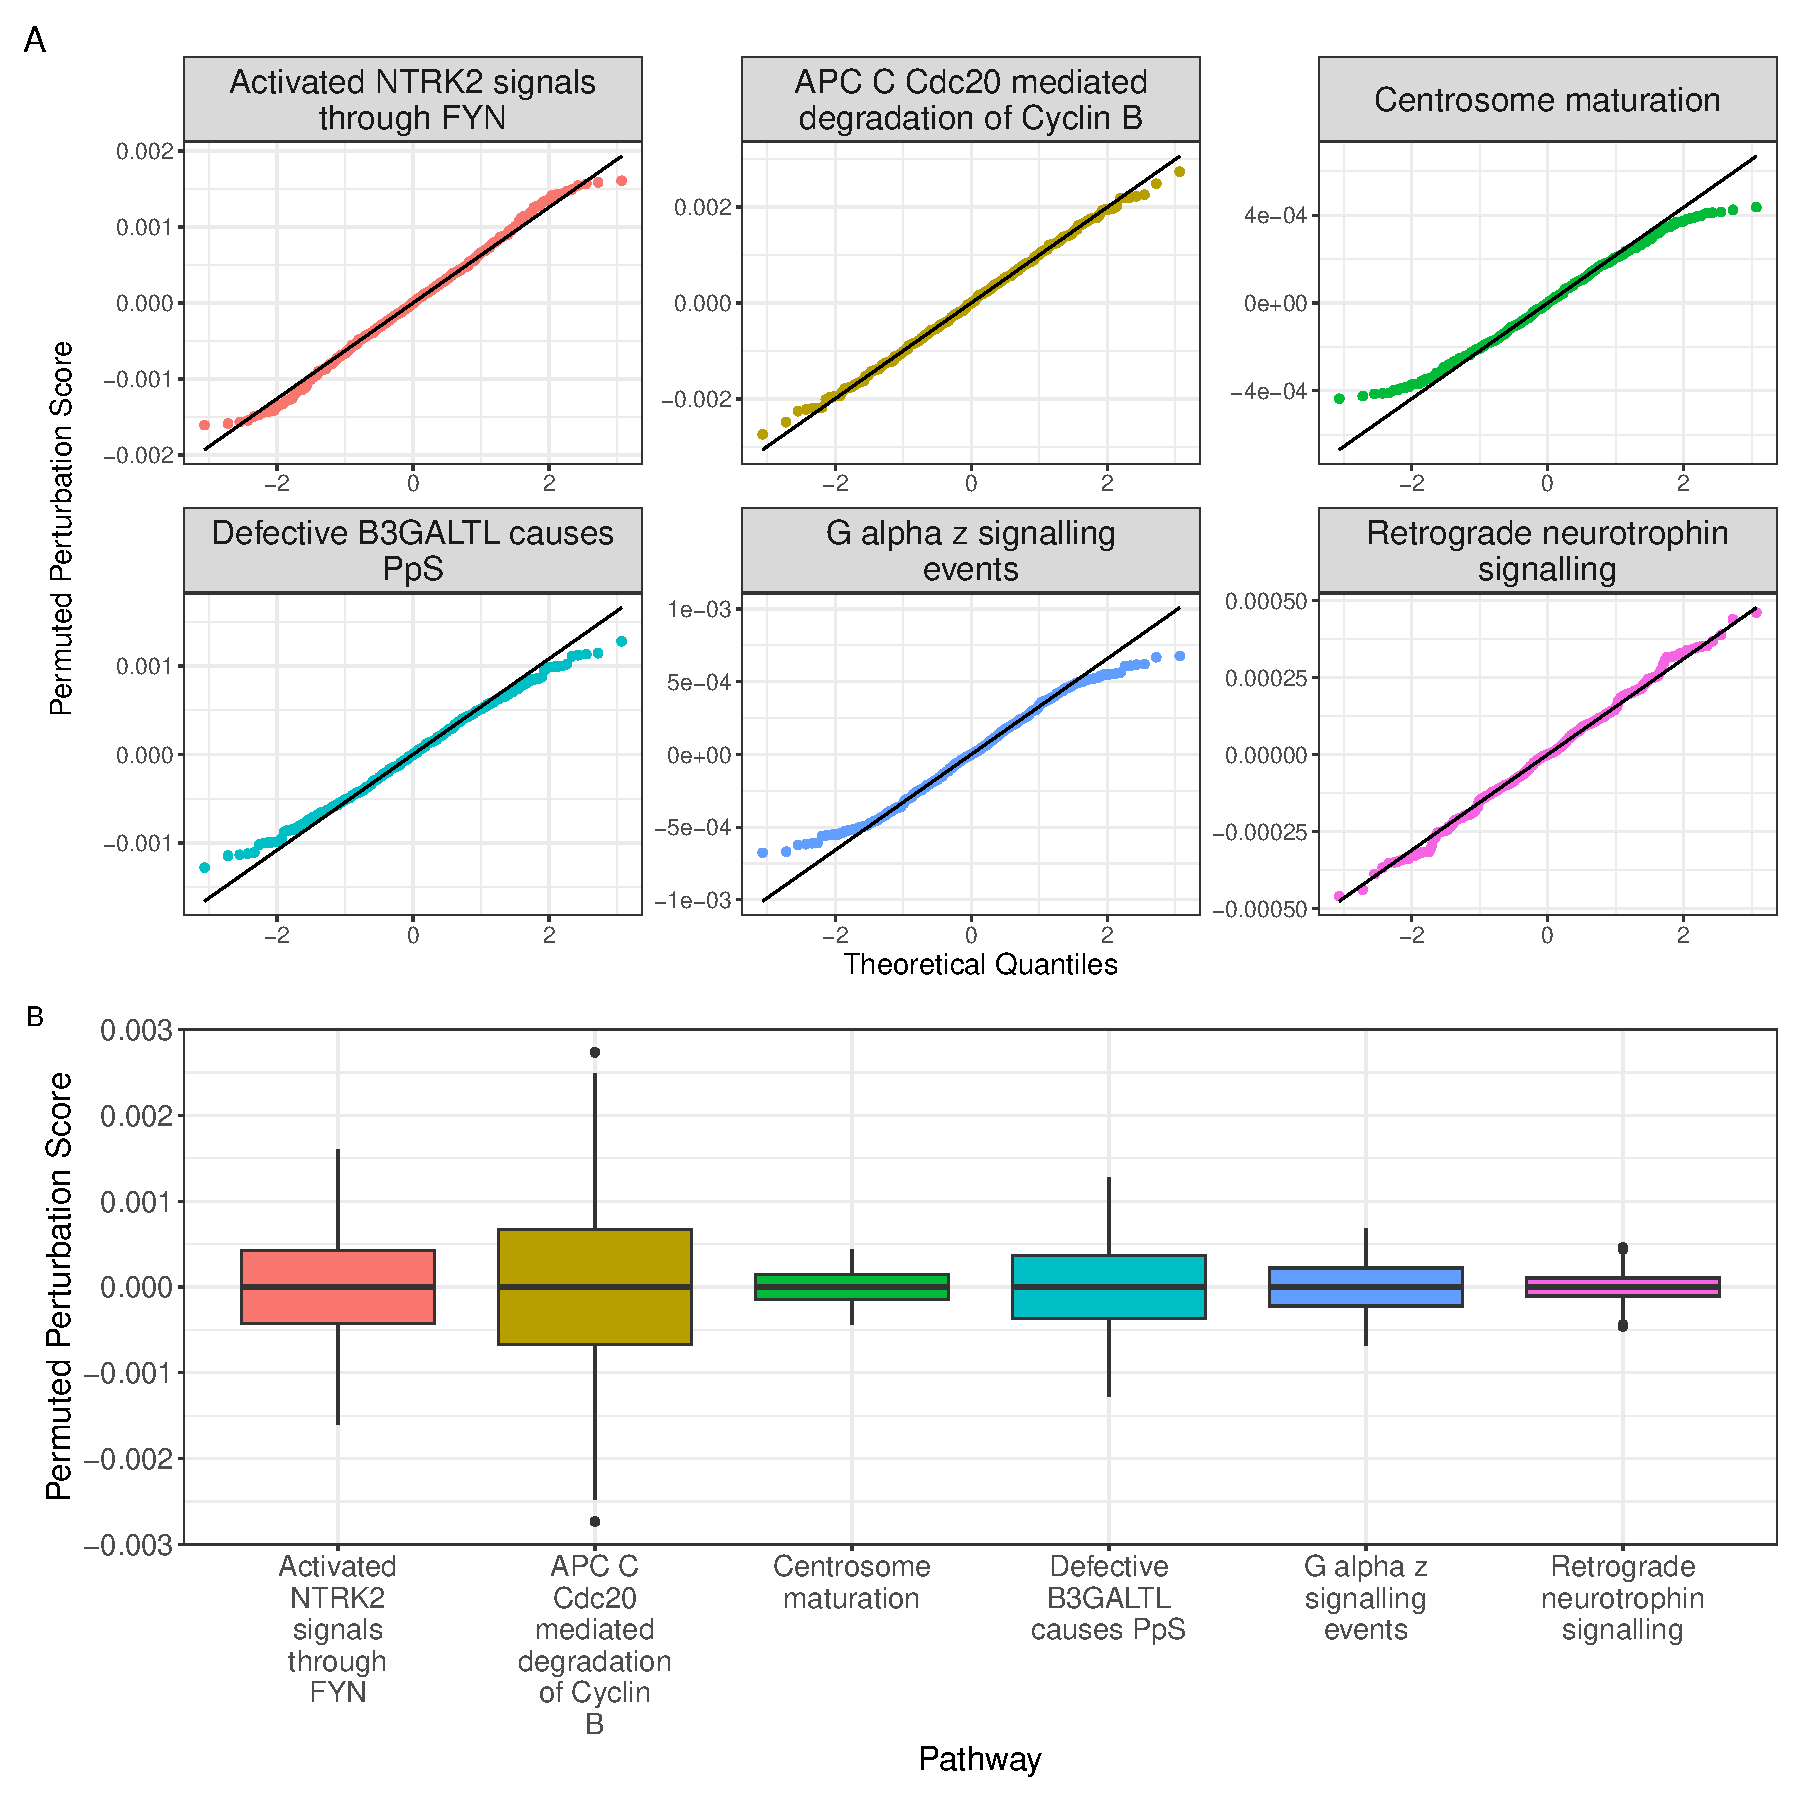
\includegraphics[width=1\linewidth]{sSNAPPY_paper_files/figure-latex/Figure3-1} 

}

\caption{(A) Q-Q plot and (B) distributions of permuted perturbation scores of six randomly selected pathways. All sampled empirical distributions are approximately normally distributed with a mean of zero.}\label{fig:Figure3}
\end{figure}

The distributions obtained from label permutations are then used to convert each pathway-level score into a robust \(Z\)-score using the function \texttt{normalise\_by\_permu()}.
Two-sided p-values for individual scores are computed based on how extreme test scores are in comparison to permuted scores for each pathway, and corrected for multiple testing using any of the available methods, returning the FDR-adjusted values by default.
In our example data, no pathways would be considered as significantly perturbed at the single-sample level using an FDR adjustment with \(\alpha\) = 0.05.

\begin{Shaded}
\begin{Highlighting}[]
\NormalTok{normalisedScores }\OtherTok{\textless{}{-}} \FunctionTok{normalise\_by\_permu}\NormalTok{(permutedScore, ssPertScore, }
                                       \AttributeTok{sortBy =} \StringTok{"pvalue"}\NormalTok{)}
\FunctionTok{head}\NormalTok{(normalisedScores)}
\end{Highlighting}
\end{Shaded}

\begin{verbatim}
##               MAD MEDIAN
## 2306 0.0006067519      0
## 2525 0.0002909911      0
## 5869 0.0001652241      0
## 5871 0.0001652241      0
## 5872 0.0001652241      0
## 7721 0.0275863198      0
##                                                           gs_name
## 2306 reactome.Golgi Cisternae Pericentriolar Stack Reorganization
## 2525       reactome.DNA Damage/Telomere Stress Induced Senescence
## 5869                        reactome.Defective CHST6 causes MCDC1
## 5871           reactome.Defective ST3GAL3 causes MCT12 and EIEE15
## 5872       reactome.Defective B4GALT1 causes B4GALT1-CDG (CDG-2d)
## 7721                        reactome.Mitochondrial protein import
##                sample         score   robustZ      pvalue adjPvalue
## 2306 EOC153_post-NACT -0.0013632057 -2.246727 0.004329004 1.0000000
## 2525 EOC153_post-NACT  0.0006149637  2.113342 0.004329004 1.0000000
## 5869 EOC349_post-NACT -0.0003304944 -2.000279 0.004329004 0.9993248
## 5871 EOC349_post-NACT -0.0003304944 -2.000279 0.004329004 0.9993248
## 5872 EOC349_post-NACT -0.0003304944 -2.000279 0.004329004 0.9993248
## 7721 EOC443_post-NACT -0.0598366717 -2.169070 0.004329004 0.9471861
\end{verbatim}

A key question of interest in our example dataset is to identify which biological processes were impacted by chemotherapy across the entire group of patients.
Using the sample-level output obtained above, we can explore this by applying t-tests or regression models across all samples.
In order to minimise spurious results, Smyth's moderated t-statistics\citep{Smyth_2004} are able to be applied across the complete dataset, with a constant variance assumed across all pathways, given that we are using Z-scores.
To perform this analysis, robust Z-scores were converted to a matrix and standard \emph{limma} methodologies were used.
For our use case here, where only one treatment group is present, no design matrix is required and a simple t-test is appropriate.

\begin{Shaded}
\begin{Highlighting}[]
\NormalTok{z\_matrix }\OtherTok{\textless{}{-}}\NormalTok{ normalisedScores }\SpecialCharTok{\%\textgreater{}\%}
\NormalTok{    dplyr}\SpecialCharTok{::}\FunctionTok{select}\NormalTok{(robustZ, gs\_name, sample) }\SpecialCharTok{\%\textgreater{}\%}
    \FunctionTok{pivot\_wider}\NormalTok{(}\AttributeTok{names\_from =} \StringTok{"sample"}\NormalTok{, }\AttributeTok{values\_from =} \StringTok{"robustZ"}\NormalTok{) }\SpecialCharTok{\%\textgreater{}\%}
    \FunctionTok{column\_to\_rownames}\NormalTok{(}\StringTok{"gs\_name"}\NormalTok{) }\SpecialCharTok{\%\textgreater{}\%}
    \FunctionTok{as.matrix}\NormalTok{()}
\NormalTok{z\_fits }\OtherTok{\textless{}{-}} \FunctionTok{lmFit}\NormalTok{(z\_matrix, }\AttributeTok{design =} \FunctionTok{rep}\NormalTok{(}\DecValTok{1}\NormalTok{, }\FunctionTok{ncol}\NormalTok{(z\_matrix))}
\NormalTok{                ) }\SpecialCharTok{\%\textgreater{}\%} 
  \FunctionTok{eBayes}\NormalTok{()}
\NormalTok{top\_table }\OtherTok{\textless{}{-}} \FunctionTok{topTable}\NormalTok{(z\_fits, }\AttributeTok{number =} \ConstantTok{Inf}\NormalTok{) }\SpecialCharTok{\%\textgreater{}\%}
  \FunctionTok{as\_tibble}\NormalTok{(}\AttributeTok{rownames =} \StringTok{"gs\_name"}\NormalTok{)}
\NormalTok{sigPathway }\OtherTok{\textless{}{-}}\NormalTok{ top\_table }\SpecialCharTok{\%\textgreater{}\%}
\NormalTok{    dplyr}\SpecialCharTok{::}\FunctionTok{filter}\NormalTok{(adj.P.Val }\SpecialCharTok{\textless{}} \FloatTok{0.05}\NormalTok{)}
\end{Highlighting}
\end{Shaded}

121 out of the 1094 tested Reactome pathways have an FDR \textless{} 0.05 in the moderated t-test, hence were considered to be significantly perturbed at the group level. The Table \ref{tab:Table1} presents the top 10 significantly inhibited and activated pathways, along with their predicted direction of change.

\begin{Shaded}
\begin{Highlighting}[]
\NormalTok{table1 }\OtherTok{\textless{}{-}}\NormalTok{ sigPathway }\SpecialCharTok{\%\textgreater{}\%}
    \FunctionTok{mutate}\NormalTok{(}
        \AttributeTok{Direction =} \FunctionTok{ifelse}\NormalTok{(logFC }\SpecialCharTok{\textless{}} \DecValTok{0}\NormalTok{, }\StringTok{"Inhibited"}\NormalTok{, }\StringTok{"Activated"}\NormalTok{), }
        \AttributeTok{gs\_name =} \FunctionTok{str\_remove\_all}\NormalTok{(gs\_name, }\StringTok{"reactome."}\NormalTok{)}
\NormalTok{    ) }\SpecialCharTok{\%\textgreater{}\%}
    \FunctionTok{split}\NormalTok{(}\AttributeTok{f =}\NormalTok{ .}\SpecialCharTok{$}\NormalTok{Direction) }\SpecialCharTok{\%\textgreater{}\%}
    \FunctionTok{lapply}\NormalTok{(}\ControlFlowTok{function}\NormalTok{(x)x[}\DecValTok{1}\SpecialCharTok{:}\DecValTok{10}\NormalTok{,]) }\SpecialCharTok{\%\textgreater{}\%}
    \FunctionTok{bind\_rows}\NormalTok{() }\SpecialCharTok{\%\textgreater{}\%}
\NormalTok{    dplyr}\SpecialCharTok{::}\FunctionTok{select}\NormalTok{(}
    \AttributeTok{Pathway =}\NormalTok{ gs\_name, }\AttributeTok{Change =}\NormalTok{ logFC,  P.Value, }\AttributeTok{FDR =}\NormalTok{ adj.P.Val, Direction}
\NormalTok{)}
\end{Highlighting}
\end{Shaded}

\begin{table}

\caption{\label{tab:Table1}Significantly impacted Reactome pathways identified among post-chemotherapy samples using sSNAPPY. Only the 10 most significantly inhibited and 10 most significantly activated pathways are shown.}
\centering
\resizebox{\linewidth}{!}{
\begin{tabular}[t]{lrrrl}
\toprule
Pathway & Change & P.Value & FDR & Direction\\
\midrule
\cellcolor{gray!6}{Signaling by Retinoic Acid} & \cellcolor{gray!6}{0.601} & \cellcolor{gray!6}{4.45e-04} & \cellcolor{gray!6}{0.0152} & \cellcolor{gray!6}{Activated}\\
Regulation of pyruvate dehydrogenase (PDH) complex & 0.598 & 4.59e-04 & 0.0152 & Activated\\
\cellcolor{gray!6}{Pyruvate metabolism} & \cellcolor{gray!6}{0.598} & \cellcolor{gray!6}{4.59e-04} & \cellcolor{gray!6}{0.0152} & \cellcolor{gray!6}{Activated}\\
Pyruvate metabolism and Citric Acid (TCA) cycle & 0.598 & 4.59e-04 & 0.0152 & Activated\\
\cellcolor{gray!6}{Negative regulation of MAPK pathway} & \cellcolor{gray!6}{0.627} & \cellcolor{gray!6}{5.40e-04} & \cellcolor{gray!6}{0.0174} & \cellcolor{gray!6}{Activated}\\
\addlinespace
Translocation of ZAP-70 to Immunological synapse & 0.624 & 8.75e-04 & 0.0218 & Activated\\
\cellcolor{gray!6}{Generation of second messenger molecules} & \cellcolor{gray!6}{0.624} & \cellcolor{gray!6}{8.75e-04} & \cellcolor{gray!6}{0.0218} & \cellcolor{gray!6}{Activated}\\
MHC class II antigen presentation & 0.628 & 1.17e-03 & 0.0241 & Activated\\
\cellcolor{gray!6}{NGF-stimulated transcription} & \cellcolor{gray!6}{0.582} & \cellcolor{gray!6}{1.36e-03} & \cellcolor{gray!6}{0.0247} & \cellcolor{gray!6}{Activated}\\
Downstream TCR signaling & 0.633 & 1.39e-03 & 0.0247 & Activated\\
\addlinespace
\cellcolor{gray!6}{Interleukin-35 Signalling} & \cellcolor{gray!6}{-0.902} & \cellcolor{gray!6}{1.69e-05} & \cellcolor{gray!6}{0.0151} & \cellcolor{gray!6}{Inhibited}\\
Sphingolipid de novo biosynthesis & -0.896 & 2.75e-05 & 0.0151 & Inhibited\\
\cellcolor{gray!6}{SUMOylation of DNA replication proteins} & \cellcolor{gray!6}{-0.819} & \cellcolor{gray!6}{6.86e-05} & \cellcolor{gray!6}{0.0152} & \cellcolor{gray!6}{Inhibited}\\
Condensation of Prometaphase Chromosomes & -0.904 & 9.91e-05 & 0.0152 & Inhibited\\
\cellcolor{gray!6}{Epigenetic regulation of gene expression} & \cellcolor{gray!6}{-0.790} & \cellcolor{gray!6}{1.21e-04} & \cellcolor{gray!6}{0.0152} & \cellcolor{gray!6}{Inhibited}\\
\addlinespace
Polo-like kinase mediated events & -0.880 & 1.43e-04 & 0.0152 & Inhibited\\
\cellcolor{gray!6}{Chromatin modifying enzymes} & \cellcolor{gray!6}{-0.791} & \cellcolor{gray!6}{1.52e-04} & \cellcolor{gray!6}{0.0152} & \cellcolor{gray!6}{Inhibited}\\
Chromatin organization & -0.791 & 1.52e-04 & 0.0152 & Inhibited\\
\cellcolor{gray!6}{SUMO E3 ligases SUMOylate target proteins} & \cellcolor{gray!6}{-0.767} & \cellcolor{gray!6}{1.83e-04} & \cellcolor{gray!6}{0.0152} & \cellcolor{gray!6}{Inhibited}\\
APC-Cdc20 mediated degradation of Nek2A & -0.838 & 2.13e-04 & 0.0152 & Inhibited\\
\bottomrule
\end{tabular}}
\end{table}

For enrichment analysis in the original study\citep{Zhang2022}, unsupervised clustering was performed on all cells labelled as cancer cells.
Clusters were then annotated manually by performing pathway enrichment testing on cluster marker genes.
Two clusters, associated with proliferative DNA repair signatures and stress-related markers, contained significantly higher numbers of post-chemotherapy cells than pre-treatment ones\citep{Zhang2022}.
The representative pathways enriched in the stress-associated cluster were \emph{IL6-mediated signaling events}, \emph{TNF signaling pathway}, and \emph{cellular responses to stress}, and the other post-chemotherapy cell dominated cluster in the original study was enriched for pathways associated with cell proliferation and DNA repair, such as the Cell cycle, DNA repair, Homology directed repair (HDR) through homologous recombination, and the Fanconi anaemia pathway.
\emph{sSNAPPY} not only detected many significant perturbed pathways that are highly concordant with the pathways reported to be enriched in the original study but also predicted their directions of changes.
For example, the DNT repair pathway \emph{SUMOylation of DNA damage response and repair proteins} pathway was predicted to be significantly inhibited by the chemotherapy.
In comparison, we also performed pathway analysis on this example dataset using two non-topological-based approaches: 1) \emph{GSEA} basing on the ranking statistics derived from the differentially expression (DE) analysis and 2) the rotation gene set testing for linear models (\emph{roast}), which does not rely on DE analysis results.
Although the \emph{SUMOylation of DNA damage response and repair proteins} pathway was also defined as significantly impacted by the chemotherapy using the two non-topological-based methods(see \href{https://github.com/Wenjun-Liu/F1000_sSNAPPY_manuscript/blob/thesis_chapter/Compare.Rmd}{extended data}), the directionality of pathway perturbation can only be predicted by \emph{sSNAPPY}.
The existing topology-based method \emph{SPIA}, on the other hand, only considers pathways containing differentially expressed genes, hence has a lower sensitivity in detecting pathway perturbation and was only able to capture changes in immune-related processes(see \href{https://github.com/Wenjun-Liu/F1000_sSNAPPY_manuscript/blob/thesis_chapter/Compare.Rmd}{extended data}).

The single-sample nature of the \emph{sSNAPPY} output also provides great flexibility: apart from considering all treated samples as biological replicates, users may elect to perform an analysis incorporating other phenotypic traits which may impact a patients responses to chemotherapy, such as disease stages or tumour grades.
To perform this step using the moderated t-statistic strategy and extend the above analysis, an appropriate design matrix is the only additional requirement for model-fitting, or alternatively, samples may be subset as may be appropriate.

\hypertarget{visualising-perturbed-pathways-as-networks}{%
\subsection{Visualising Perturbed Pathways as Networks}\label{visualising-perturbed-pathways-as-networks}}

A valuable feature of sSNAPPY is the provision of several visualisation functions to assist in the interpretation of results.
Biological pathways are not independent of each other with many genes playing a role across multiple pathways, and as such, viewing pathway analysis results as a network can be a powerful way to intuitively summarise the results and facilitate interpretation of the underlying biology.
The \texttt{plot\_gs\_network()} function allows users to easily convert a list of relevant biological pathways to a network where edges between pathway nodes represent overlapping genes.
Defined by the colorBy parameter, pathway nodes can be coloured by either the predicted direction of change or by significance levels (Figure \ref{fig:Figure4}).
The returned plot is a ggplot2 \citep{Wickham2009} object, meaning that components of the plotting theme and other parameters can be customized as for any other ggplot2 objects.

In the following example, we'll inspect the 10 most significantly inhibited and 10 most significantly activated pathways, which involved four steps to prepare the data: 1) rename the logFC column to reflect the true meaning of the value and, 2) create a categorical variable with the pathway status, 3) transform p-values for simpler visualisation and 4) obtain a subset of pathways to visualise.

\begin{Shaded}
\begin{Highlighting}[]
\NormalTok{sigPathway }\OtherTok{\textless{}{-}}\NormalTok{ sigPathway }\SpecialCharTok{\%\textgreater{}\%}
\NormalTok{    dplyr}\SpecialCharTok{::}\FunctionTok{rename}\NormalTok{(}\AttributeTok{Z =}\NormalTok{ logFC) }\SpecialCharTok{\%\textgreater{}\%} 
    \FunctionTok{mutate}\NormalTok{(}
        \AttributeTok{status =} \FunctionTok{ifelse}\NormalTok{(}
\NormalTok{            Z }\SpecialCharTok{\textgreater{}} \DecValTok{0}\NormalTok{, }\StringTok{"Activated"}\NormalTok{, }\StringTok{"Inhibited"}\NormalTok{), }
        \AttributeTok{status =} \FunctionTok{ifelse}\NormalTok{(}
\NormalTok{            adj.P.Val }\SpecialCharTok{\textless{}} \FloatTok{0.05}\NormalTok{, status, }\StringTok{"Unchanged"}
\NormalTok{        ), }
        \AttributeTok{status =} \FunctionTok{as.factor}\NormalTok{(status),}
        \StringTok{\textasciigrave{}}\AttributeTok{{-}log10(p)}\StringTok{\textasciigrave{}} \OtherTok{=} \SpecialCharTok{{-}}\FunctionTok{log10}\NormalTok{(P.Value)}
\NormalTok{    )  }\SpecialCharTok{\%\textgreater{}\%} 
    \FunctionTok{split}\NormalTok{(}\AttributeTok{f =}\NormalTok{ .}\SpecialCharTok{$}\NormalTok{status) }\SpecialCharTok{\%\textgreater{}\%}
    \FunctionTok{lapply}\NormalTok{(}\ControlFlowTok{function}\NormalTok{(x)x[}\DecValTok{1}\SpecialCharTok{:}\DecValTok{10}\NormalTok{,]) }\SpecialCharTok{\%\textgreater{}\%}
    \FunctionTok{bind\_rows}\NormalTok{()}
\end{Highlighting}
\end{Shaded}

\begin{Shaded}
\begin{Highlighting}[]
\FunctionTok{set.seed}\NormalTok{(}\DecValTok{123}\NormalTok{)}
\CommentTok{\# Plot the network structure}
\NormalTok{p1 }\OtherTok{\textless{}{-}} \FunctionTok{plot\_gs\_network}\NormalTok{(}
  \AttributeTok{normalisedScores =}\NormalTok{ sigPathway, }\AttributeTok{gsTopology =}\NormalTok{ gsTopology, }\AttributeTok{colorBy =} \StringTok{"status"}\NormalTok{,}
  \AttributeTok{gsNameSize =} \DecValTok{3}
\NormalTok{) }\SpecialCharTok{+}
  \FunctionTok{scale\_colour\_manual}\NormalTok{(}\AttributeTok{values =} \FunctionTok{c}\NormalTok{(}\StringTok{"red"}\NormalTok{, }\StringTok{"blue"}\NormalTok{, }\StringTok{"grey30"}\NormalTok{)) }\SpecialCharTok{+}
  \FunctionTok{theme\_void}\NormalTok{() }\SpecialCharTok{+}
  \FunctionTok{theme}\NormalTok{(}\AttributeTok{legend.text =} \FunctionTok{element\_text}\NormalTok{(}\AttributeTok{size =} \DecValTok{10}\NormalTok{)) }
\FunctionTok{set.seed}\NormalTok{(}\DecValTok{123}\NormalTok{)}
\NormalTok{p2 }\OtherTok{\textless{}{-}} \FunctionTok{plot\_gs\_network}\NormalTok{(}
  \AttributeTok{normalisedScores =}\NormalTok{ sigPathway,}
  \AttributeTok{gsTopology =}\NormalTok{ gsTopology, }
  \AttributeTok{colorBy  =} \StringTok{"{-}log10(p)"}\NormalTok{, }
  \AttributeTok{gsNameSize =} \DecValTok{3}\NormalTok{,}
  \AttributeTok{gsLegTitle =} \FunctionTok{expression}\NormalTok{(}\FunctionTok{paste}\NormalTok{(}\SpecialCharTok{{-}}\NormalTok{log[}\DecValTok{10}\NormalTok{], }\StringTok{"p"}\NormalTok{))}
\NormalTok{) }\SpecialCharTok{+}
  \FunctionTok{scale\_colour\_viridis\_c}\NormalTok{() }\SpecialCharTok{+}
  \FunctionTok{theme\_void}\NormalTok{() }\SpecialCharTok{+}
  \FunctionTok{theme}\NormalTok{(}
    \AttributeTok{legend.text =} \FunctionTok{element\_text}\NormalTok{(}\AttributeTok{size =} \DecValTok{8}\NormalTok{),}
    \AttributeTok{legend.title =} \FunctionTok{element\_text}\NormalTok{(}\AttributeTok{size =} \DecValTok{10}\NormalTok{)}
\NormalTok{  ) }
\NormalTok{p1 }\SpecialCharTok{/}\NormalTok{ p2 }\SpecialCharTok{+} \FunctionTok{plot\_annotation}\NormalTok{(}\AttributeTok{tag\_levels =} \StringTok{"A"}\NormalTok{) }
\end{Highlighting}
\end{Shaded}

\begin{figure}

{\centering 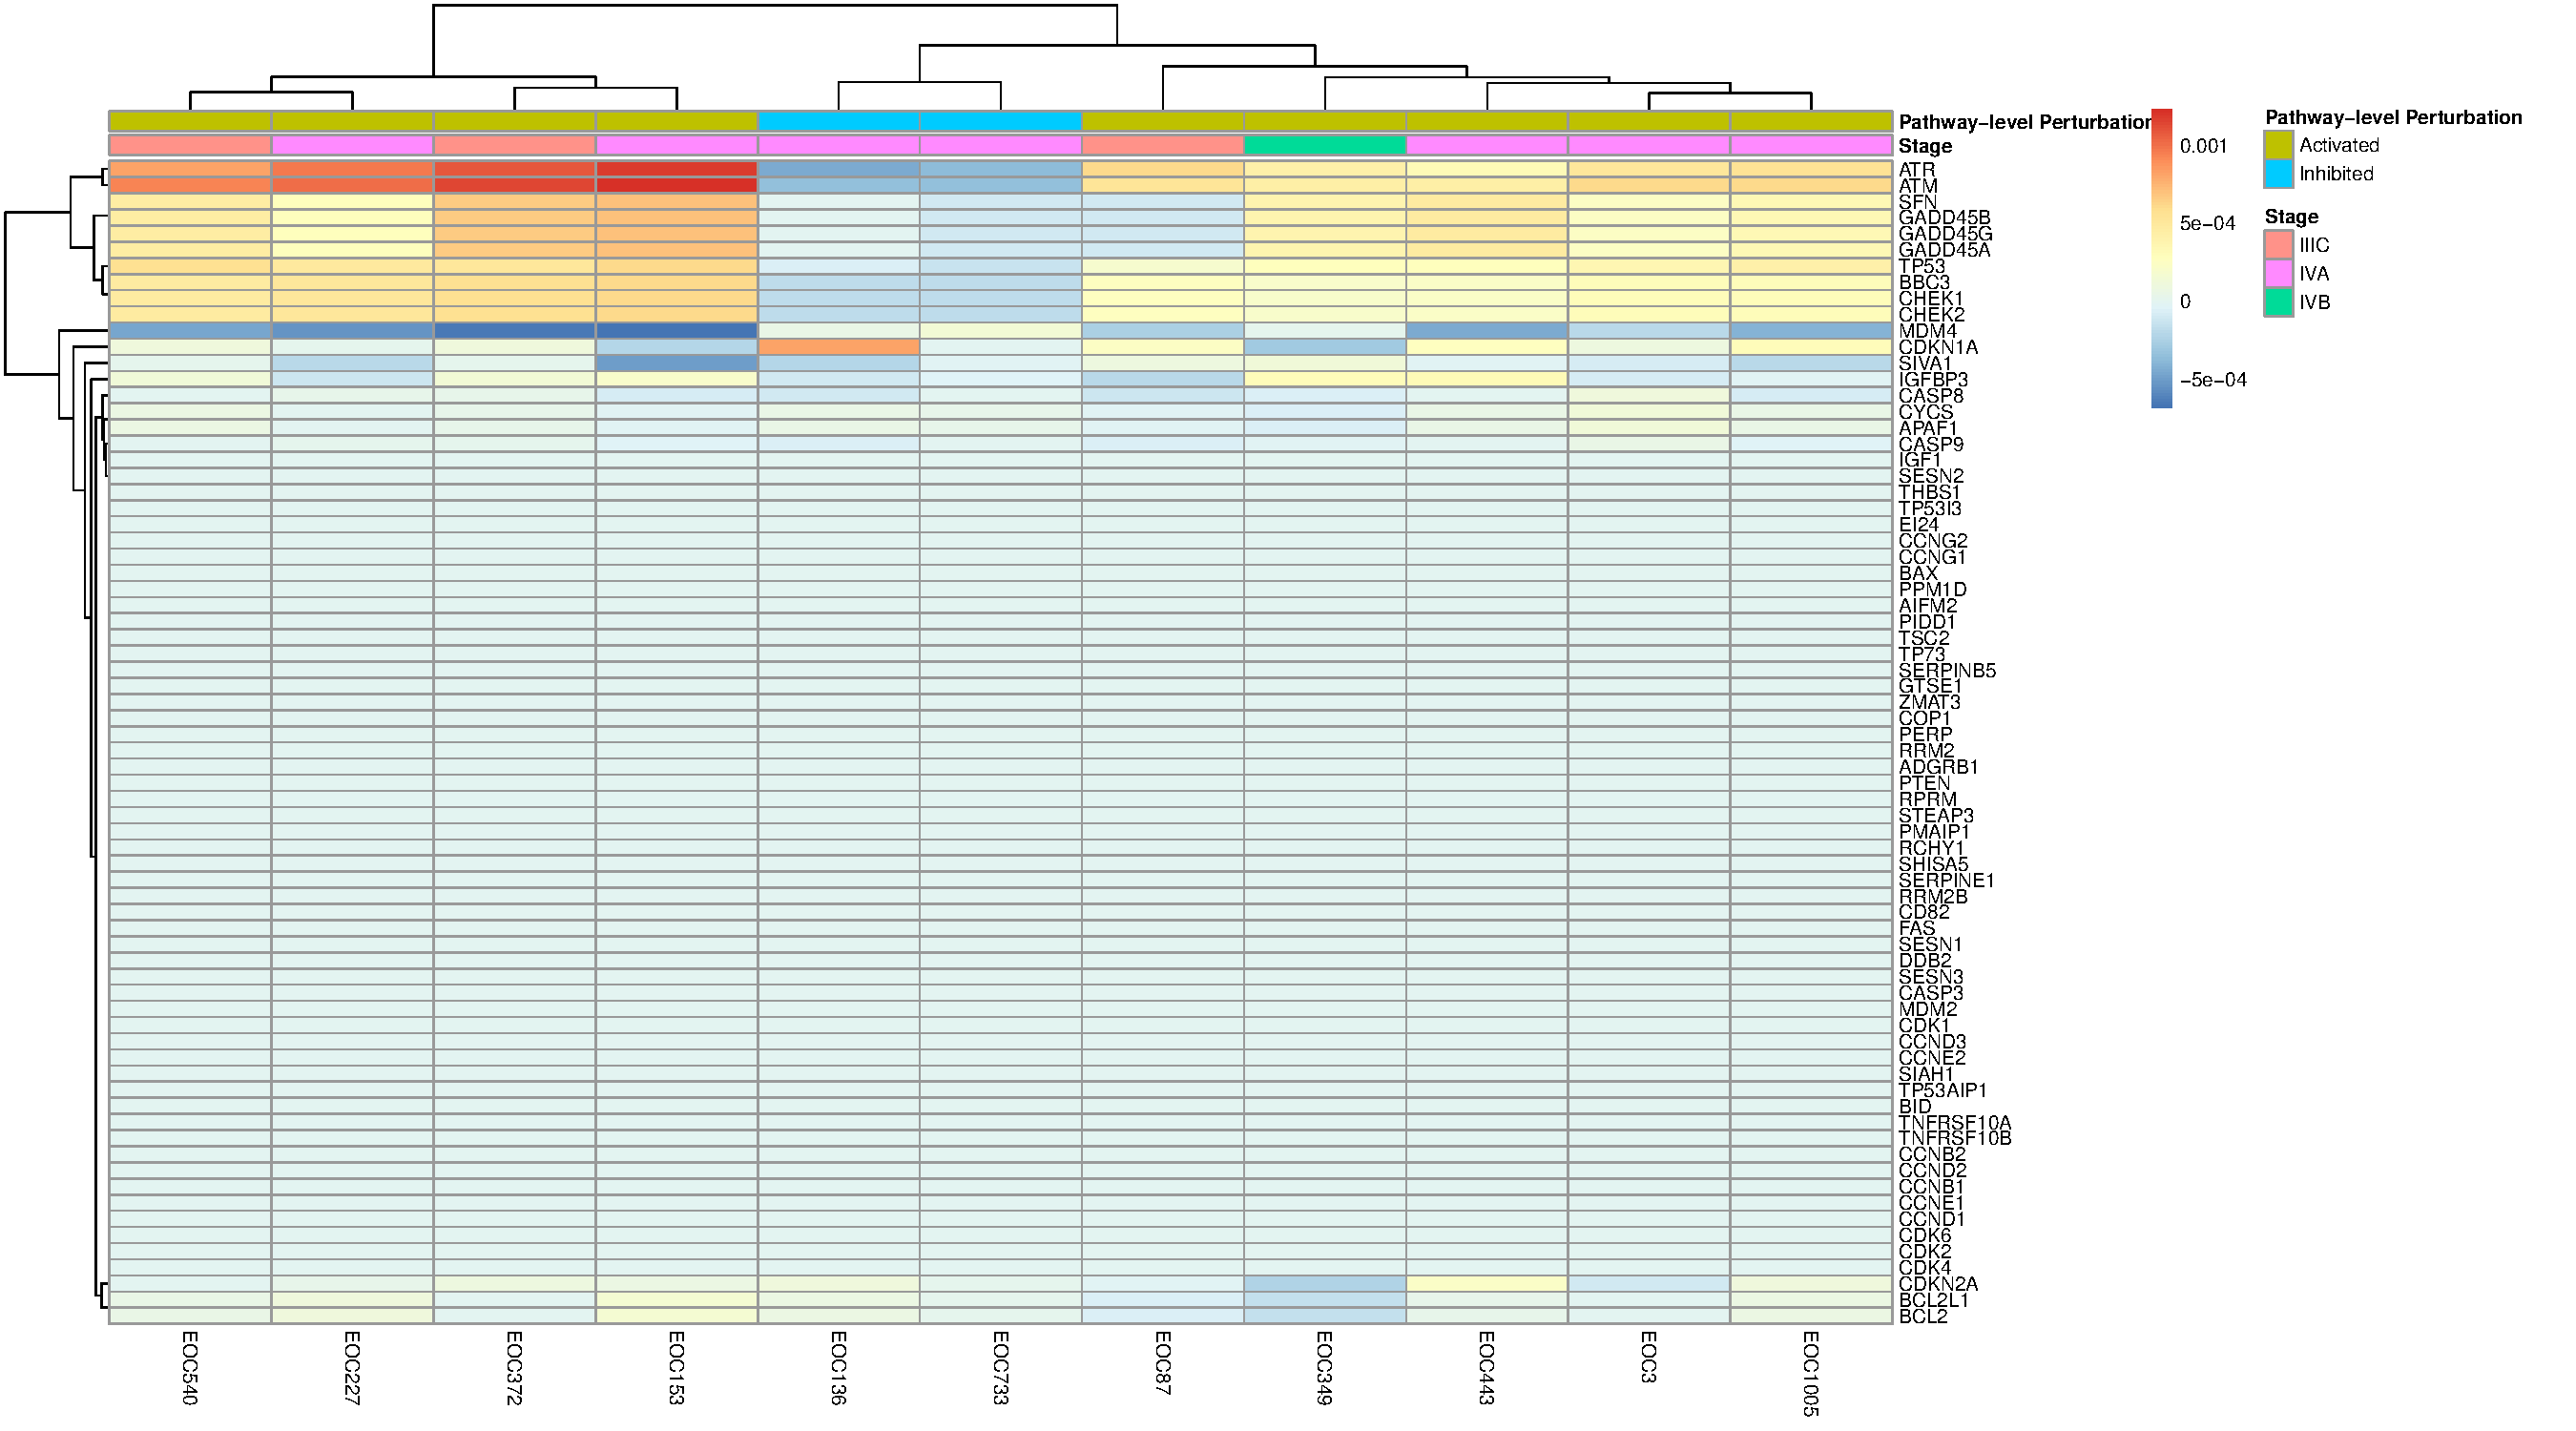
\includegraphics[width=1\linewidth]{sSNAPPY_paper_files/figure-latex/Figure4-1} 

}

\caption{Significantly perturbed Reactome pathways identified among post-chemotherapy samples using sSNAPPY, colored by (A) predicted direction of changes and (B) -log10(p-values). Only the 10 most significantly inhibited and 10 most significantly activated pathways are shown.}\label{fig:Figure4}
\end{figure}

An advantage of visualising pathway analysis results using network structures is that it allows the identification of highly connected pathways (Figure \ref{fig:Figure4}).
To summarise related pathways and further enable interpretation, we can apply community detection\citep{Newman2004} to group related pathways into `communities'.
sSNAPPY's \texttt{plot\_community()} function is a ``one-stop shop'' for applying a community detection algorithm of the user's choice to the network structure and annotating identified communities by the most common pathway category, denoting the main biological processes perturbed in that community.
The most recent categories for both KEGG and Reactome databases were curated from their respective website (\href{https://www.genome.jp/kegg/pathway.html}{KEGG website} \& \href{https://reactome.org/PathwayBrowser/\#/R-HSA-1632852&PATH=R-HSA-9612973}{Reactome website}) and included as parts of sSNAPPY.
Analyses involving other pathway databases may require user-provided pathway categories.
When the information about pathway categorisations is available, annotation of pathway communities is automatically completed.
In the current dataset, the Louvain method was applied to the network of biological pathways and revealed five primary communities: 1) Adaptive Immune System; 2) Cell Cycle, Mitotic; 3) Chromatin modifying enzymes \& Epigenetic regulation of gene expression; 4) Post-translational protein modification and 5) The citric acid (TCA) cycle and respiratory electron transport (Figure \ref{fig:Figure5}).
The largest community formed was the Adaptive Immune System pathway, indicating a clear immune-signalling aspect to these results.

\begin{Shaded}
\begin{Highlighting}[]
\FunctionTok{load}\NormalTok{(}\FunctionTok{system.file}\NormalTok{(}\StringTok{"extdata"}\NormalTok{, }\StringTok{"gsAnnotation\_df\_reactome.rda"}\NormalTok{, }\AttributeTok{package =} \StringTok{"sSNAPPY"}\NormalTok{))}
\FunctionTok{set.seed}\NormalTok{(}\DecValTok{456}\NormalTok{)}
\FunctionTok{plot\_community}\NormalTok{(}
    \AttributeTok{normalisedScores =}\NormalTok{ sigPathway,}
    \AttributeTok{gsTopology =}\NormalTok{ gsTopology, }
    \AttributeTok{gsAnnotation =}\NormalTok{ gsAnnotation\_df\_reactome,}
    \AttributeTok{colorBy =} \StringTok{"status"}\NormalTok{,}
    \AttributeTok{lb\_size =} \DecValTok{3}
\NormalTok{) }\SpecialCharTok{+}
    \FunctionTok{scale\_colour\_manual}\NormalTok{(}\AttributeTok{values =} \FunctionTok{c}\NormalTok{(}\StringTok{"red"}\NormalTok{, }\StringTok{"blue"}\NormalTok{)) }\SpecialCharTok{+}
    \FunctionTok{scale\_fill\_viridis\_d}\NormalTok{() }\SpecialCharTok{+}
    \FunctionTok{scale\_x\_continuous}\NormalTok{(}\AttributeTok{expand =} \FunctionTok{expansion}\NormalTok{(}\FloatTok{0.25}\NormalTok{)) }\SpecialCharTok{+}
    \FunctionTok{scale\_y\_continuous}\NormalTok{(}\AttributeTok{expand =} \FunctionTok{expansion}\NormalTok{(}\FloatTok{0.25}\NormalTok{)) }\SpecialCharTok{+}
    \FunctionTok{guides}\NormalTok{(}\AttributeTok{fill =} \ConstantTok{FALSE}\NormalTok{) }\SpecialCharTok{+}
    \FunctionTok{theme\_void}\NormalTok{() }\SpecialCharTok{+}
    \FunctionTok{theme}\NormalTok{(}
        \AttributeTok{legend.text =} \FunctionTok{element\_text}\NormalTok{(}\AttributeTok{size =} \DecValTok{8}\NormalTok{),}
        \AttributeTok{legend.title =} \FunctionTok{element\_text}\NormalTok{(}\AttributeTok{size =} \DecValTok{10}\NormalTok{)}
\NormalTok{    )}
\end{Highlighting}
\end{Shaded}

\begin{verbatim}
## Warning: The `<scale>` argument of `guides()` cannot be `FALSE`. Use "none" instead as
## of ggplot2 3.3.4.
## This warning is displayed once every 8 hours.
## Call `lifecycle::last_lifecycle_warnings()` to see where this warning was
## generated.
\end{verbatim}

\begin{figure}

{\centering 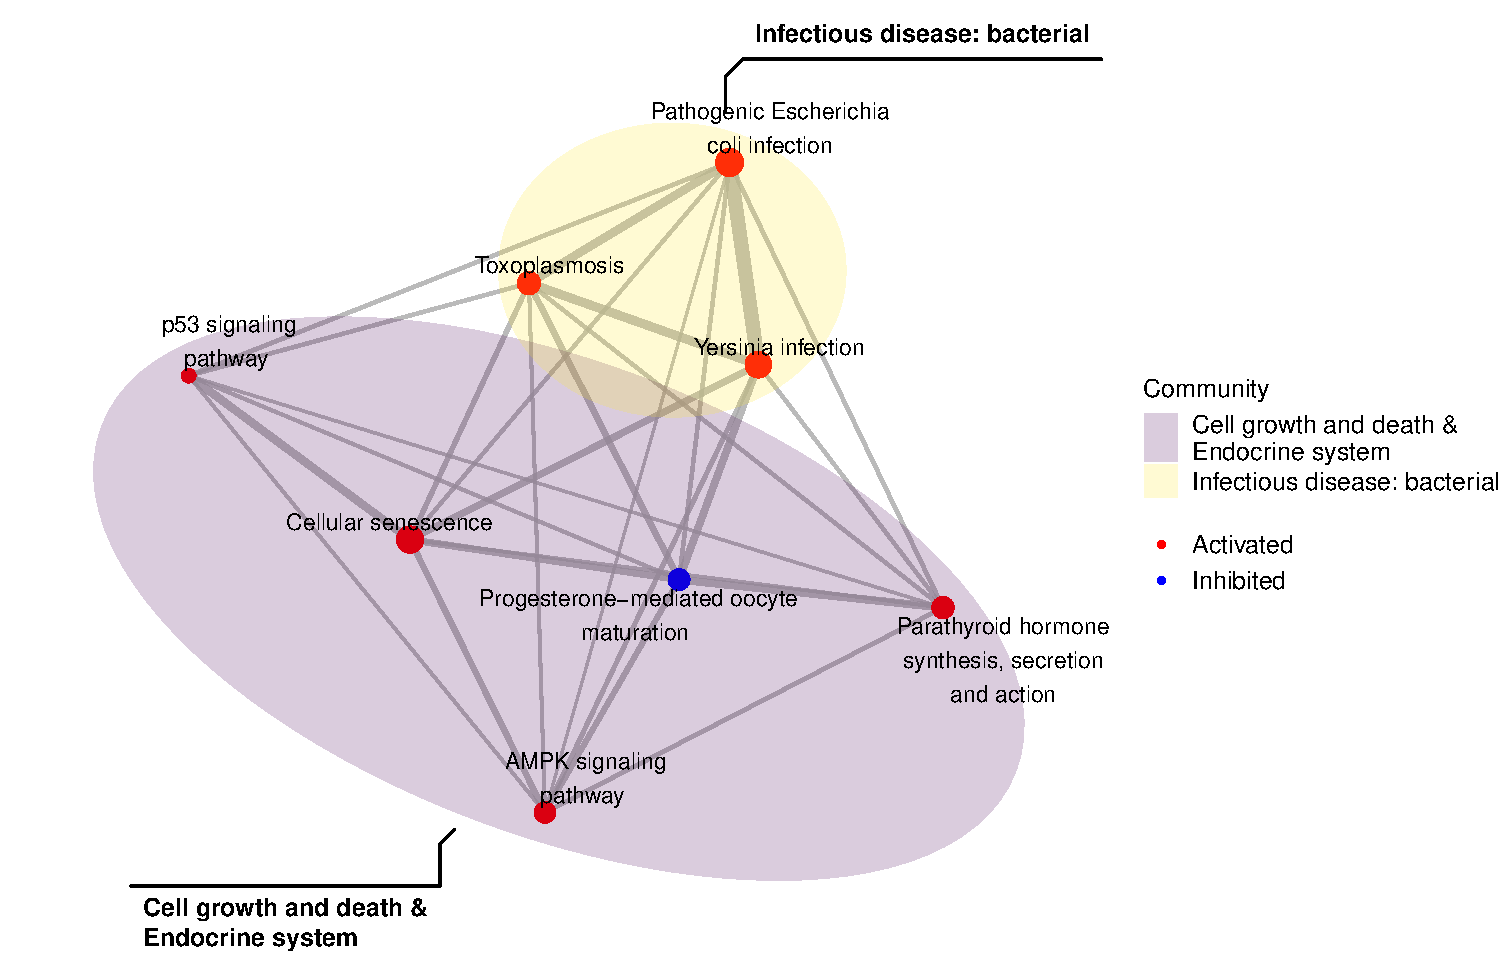
\includegraphics[width=1\linewidth]{sSNAPPY_paper_files/figure-latex/Figure5-1} 

}

\caption{Significantly perturbed Reactome pathways identified among post-chemotherapy samples using sSNAPPY, colored by community structures detected through the louvain algorithm. The main biological processes associated with the top 20 pathways that wer most perturbed by the chemotherapy were shown.}\label{fig:Figure5}
\end{figure}

A key advantage of sSNAPPY is that it does not require the prior identification of differentially expressed genes, as this is a common challenge within clinical datasets.
However, knowing which genes are implicated in the perturbation of pathways, particularly those which influence multiple pathways, can provide valuable insights for hypothesis generation and the underlying biological mechanisms.
Therefore, sSNAPPY provides another visualisation feature called \texttt{plot\_gs2gene}, which enables the inclusion of select genes from each pathway using network structures.
Users can provide a vector of fold-change estimates to visualise genes within pathways, showing their estimated change in expression.
As pathways often include hundreds of genes, it is recommended to filter for genes most likely to be playing a significant role.
In this example dataset, only genes within the top 500 when ranking by the magnitude of the mean log fold-change were included (Figure \ref{fig:Figure6}).
An alternative strategy will be to select genes based on test-statistics, however, this decision is up to the individual researcher.

\begin{Shaded}
\begin{Highlighting}[]
\NormalTok{meanFC }\OtherTok{\textless{}{-}} \FunctionTok{rowMeans}\NormalTok{(weightedFC}\SpecialCharTok{$}\NormalTok{weighted\_logFC) }\SpecialCharTok{/}\NormalTok{ weightedFC}\SpecialCharTok{$}\NormalTok{weight}
\NormalTok{top500 }\OtherTok{\textless{}{-}} \FunctionTok{rank}\NormalTok{(}\DecValTok{1}\SpecialCharTok{/}\FunctionTok{abs}\NormalTok{(meanFC)) }\SpecialCharTok{\textless{}=} \DecValTok{500}
\NormalTok{dirFC }\OtherTok{\textless{}{-}} \FunctionTok{ifelse}\NormalTok{(meanFC }\SpecialCharTok{\textgreater{}} \DecValTok{0}\NormalTok{, }\StringTok{"Up{-}Regulated"}\NormalTok{, }\StringTok{"Down{-}Regulated"}\NormalTok{)}
\end{Highlighting}
\end{Shaded}

Since Reactome pathway topologies were retrieved using Entrez IDs, users can provide a data.frame mapping Entrez IDs to their chosen identifiers, such as gene names, through the mapEntrezID parameter, in order to make the visualisations more informative.
A data.frame converting Entrez IDs to Ensembl gene names was derived from the Ensembl Release 101\citep{Ensembl2022} and has been made available as part of the package and serves as a helpful template for future mapping operations by users.

\begin{Shaded}
\begin{Highlighting}[]
\FunctionTok{load}\NormalTok{(}\FunctionTok{system.file}\NormalTok{(}\StringTok{"extdata"}\NormalTok{, }\StringTok{"entrez2name.rda"}\NormalTok{, }\AttributeTok{package =} \StringTok{"sSNAPPY"}\NormalTok{))}
\FunctionTok{head}\NormalTok{(entrez2name)}
\end{Highlighting}
\end{Shaded}

\begin{verbatim}
## # A tibble: 6 x 2
##   entrezid           mapTo                   
##   <chr>              <chr>                   
## 1 ENTREZID:84771     DDX11L1                 
## 2 ENTREZID:727856    DDX11L1/DDX11L9/DDX11L10
## 3 ENTREZID:100287102 DDX11L1                 
## 4 ENTREZID:100287596 DDX11L1/DDX11L9         
## 5 ENTREZID:102725121 DDX11L1                 
## 6 ENTREZID:653635    WASH7P
\end{verbatim}

\begin{Shaded}
\begin{Highlighting}[]
\FunctionTok{set.seed}\NormalTok{(}\DecValTok{123}\NormalTok{)}
\FunctionTok{plot\_gs2gene}\NormalTok{(}
    \AttributeTok{normalisedScores =}\NormalTok{ sigPathway, }
    \AttributeTok{gsTopology =}\NormalTok{ gsTopology, }
    \AttributeTok{colorGsBy =} \StringTok{"status"}\NormalTok{, }
    \AttributeTok{mapEntrezID =}\NormalTok{ entrez2name, }
    \AttributeTok{geneFC =}\NormalTok{ meanFC[top500], }
    \AttributeTok{layout =} \StringTok{"kk"}\NormalTok{,}
    \AttributeTok{edgeAlpha =} \DecValTok{1}\NormalTok{, }
    \AttributeTok{gsNameSize =} \DecValTok{4}\NormalTok{, }
    \AttributeTok{gsNodeSize =} \DecValTok{4}\NormalTok{,}
    \AttributeTok{geneNameSize =} \DecValTok{4}
\NormalTok{) }\SpecialCharTok{+}
    \FunctionTok{scale\_colour\_gradient2}\NormalTok{(}\AttributeTok{name =} \StringTok{"logFC"}\NormalTok{) }\SpecialCharTok{+}
    \FunctionTok{scale\_fill\_manual}\NormalTok{(}\AttributeTok{values =} \FunctionTok{c}\NormalTok{(}\StringTok{"red"}\NormalTok{, }\StringTok{"blue"}\NormalTok{, }\StringTok{"grey50"}\NormalTok{)) }\SpecialCharTok{+}
    \FunctionTok{theme\_void}\NormalTok{() }\SpecialCharTok{+}
    \FunctionTok{theme}\NormalTok{(}
        \AttributeTok{legend.text =} \FunctionTok{element\_text}\NormalTok{(}\AttributeTok{size =} \DecValTok{12}\NormalTok{),}
        \AttributeTok{legend.title =} \FunctionTok{element\_text}\NormalTok{(}\AttributeTok{size =} \DecValTok{12}\NormalTok{)}
\NormalTok{    )}
\end{Highlighting}
\end{Shaded}

\begin{figure}

{\centering 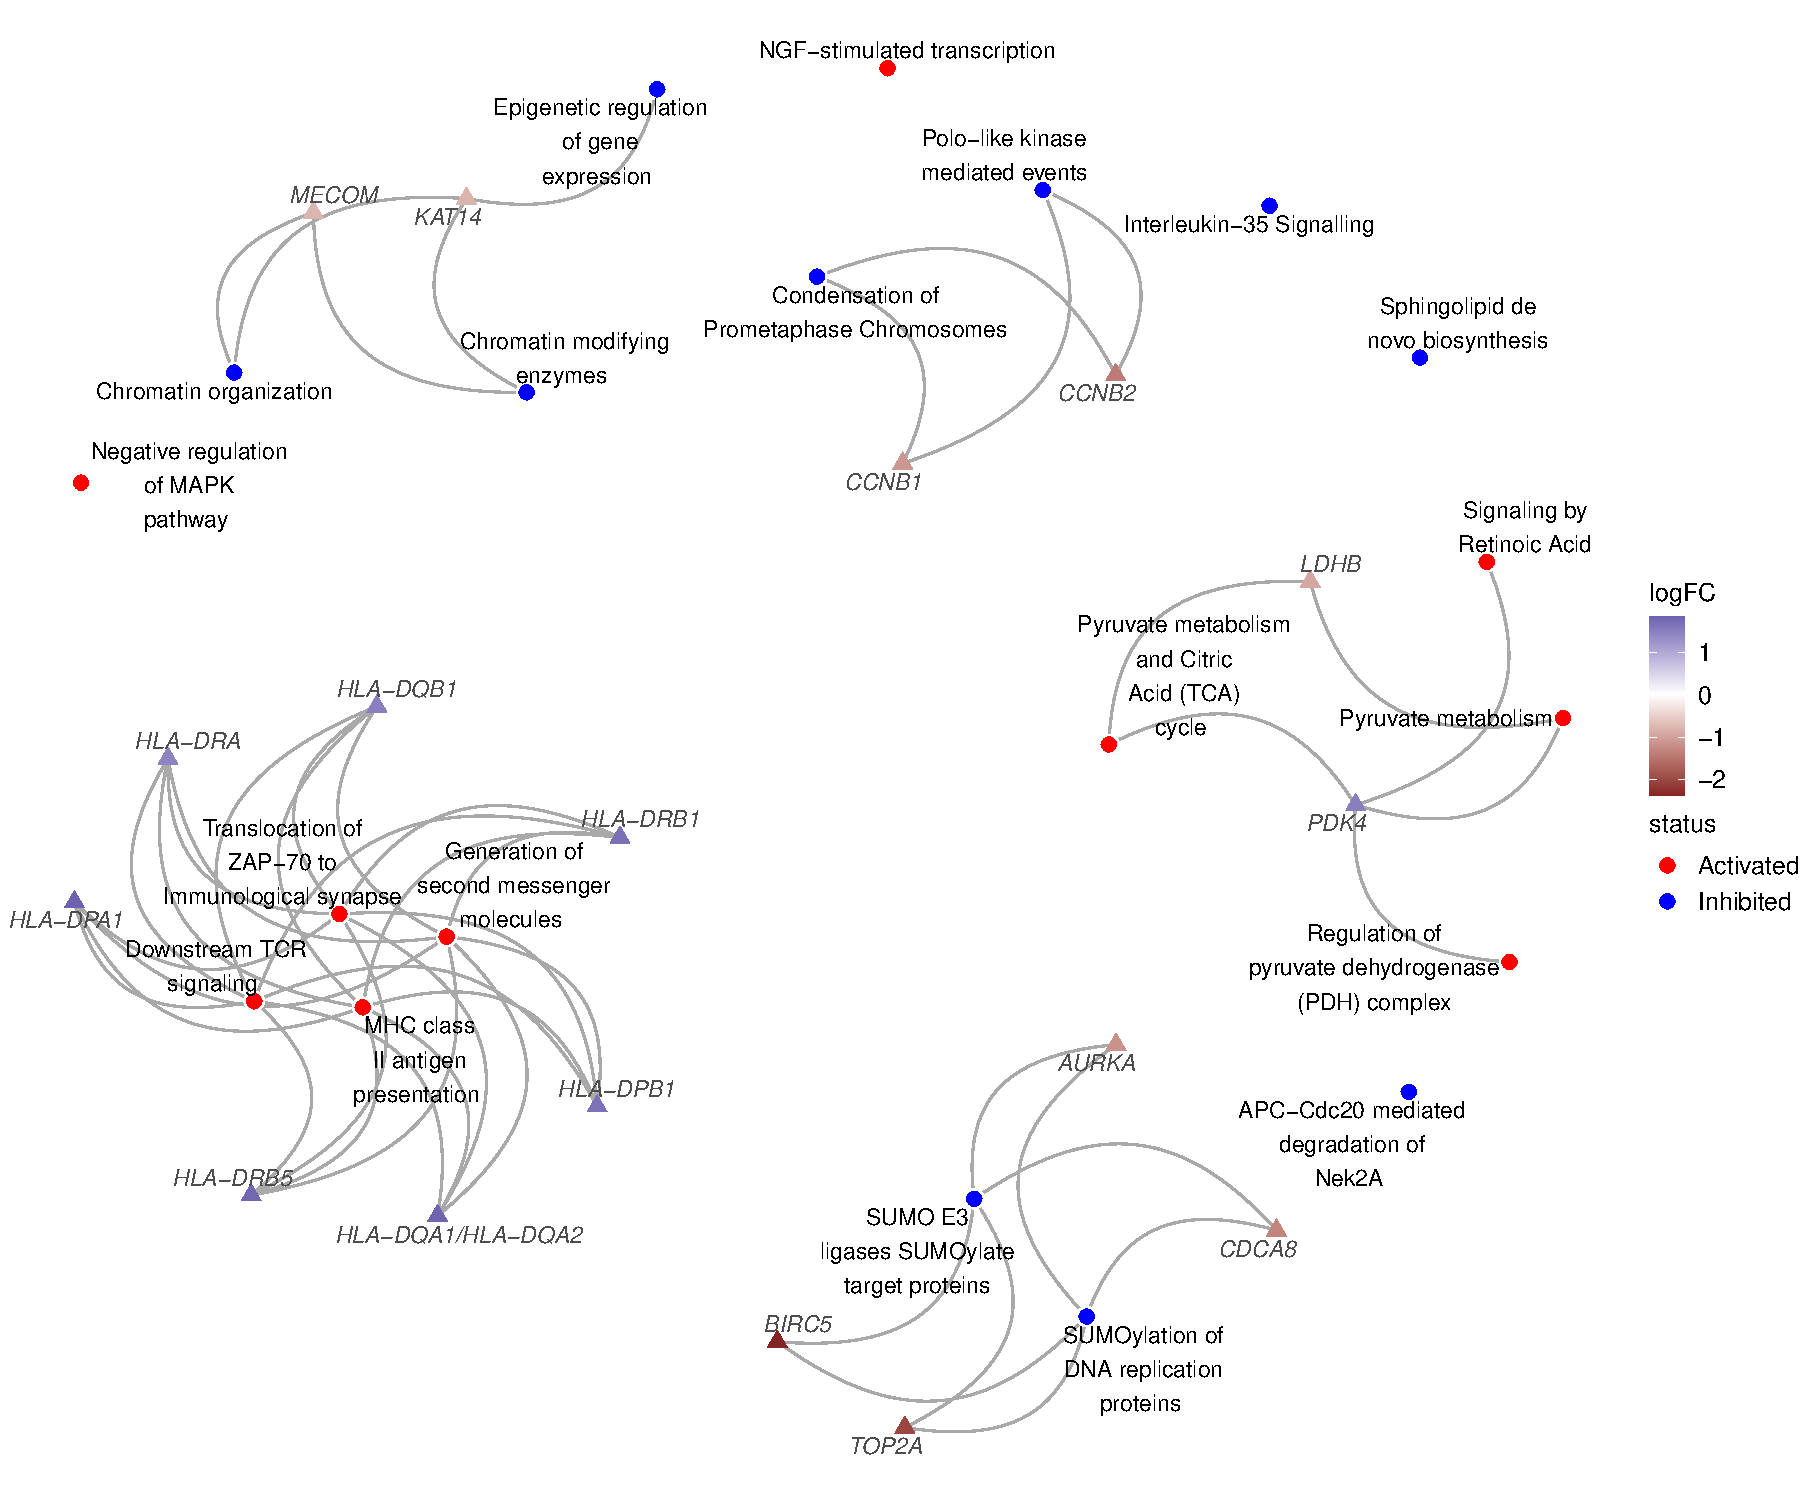
\includegraphics[width=1\linewidth]{sSNAPPY_paper_files/figure-latex/Figure6-1} 

}

\caption{Significantly perturbed Reactome pathways identified among post-chemotherapy samples using sSNAPPY, showing any genes in the top 500 ranked by magnitude of change in expression, and which pathways they are likely contributing to. Only the 10 most significantly inhibited and 10 most significantly activated pathways are shown.}\label{fig:Figure6}
\end{figure}

\hypertarget{identifying-key-gene-contributions}{%
\subsection{Identifying Key Gene Contributions}\label{identifying-key-gene-contributions}}

To further investigate a specific pathway and elucidate which are the key genes contributing to the final perturbation score, we can generate a heatmap via \texttt{plot\_gene\_contribution()} which shows the gene-level perturbation scores for the top-ranked members of a given pathway.
This function takes advantage of the plotting capabilities of the \texttt{pheatmap} package\citep{pheatmap}, and as such, other annotations are also able to be easily included, such as patient response, or which general ranges the pathway-level normalised Z-Scores are in.
Inclusion of the Z-Scores enabled the assessment of the level of perturbation predicted in each sample and key genes involved (Figure \ref{fig:Figure7}).

\begin{Shaded}
\begin{Highlighting}[]
\NormalTok{annotation\_df }\OtherTok{\textless{}{-}}\NormalTok{ normalisedScores }\SpecialCharTok{\%\textgreater{}\%}
\NormalTok{    dplyr}\SpecialCharTok{::}\FunctionTok{filter}\NormalTok{(gs\_name }\SpecialCharTok{==} \StringTok{"reactome.SUMOylation of DNA replication proteins"}\NormalTok{) }\SpecialCharTok{\%\textgreater{}\%}
    \FunctionTok{left\_join}\NormalTok{(dplyr}\SpecialCharTok{::}\FunctionTok{select}\NormalTok{(sample\_meta, sample,  CRS), }\AttributeTok{by =} \StringTok{"sample"}\NormalTok{) }\SpecialCharTok{\%\textgreater{}\%}
    \FunctionTok{mutate}\NormalTok{(}
      \StringTok{\textasciigrave{}}\AttributeTok{Z Range}\StringTok{\textasciigrave{}} \OtherTok{=} \FunctionTok{cut}\NormalTok{(}
\NormalTok{        robustZ, }\AttributeTok{breaks =} \FunctionTok{seq}\NormalTok{(}\SpecialCharTok{{-}}\DecValTok{2}\NormalTok{, }\DecValTok{2}\NormalTok{, }\AttributeTok{length.out =} \DecValTok{6}\NormalTok{), }\AttributeTok{include.lowest =} \ConstantTok{TRUE}
\NormalTok{      ), }
      \AttributeTok{sample =} \FunctionTok{str\_remove\_all}\NormalTok{(sample, }\StringTok{"\_post{-}NACT"}\NormalTok{)}
\NormalTok{    ) }\SpecialCharTok{\%\textgreater{}\%} 
\NormalTok{    dplyr}\SpecialCharTok{::}\FunctionTok{select}\NormalTok{(sample, }\StringTok{\textasciigrave{}}\AttributeTok{Z Range}\StringTok{\textasciigrave{}}\NormalTok{, CRS)  }
\NormalTok{z\_levels }\OtherTok{\textless{}{-}} \FunctionTok{levels}\NormalTok{(annotation\_df}\SpecialCharTok{$}\StringTok{\textasciigrave{}}\AttributeTok{Z Range}\StringTok{\textasciigrave{}}\NormalTok{)}
\NormalTok{annotation\_col }\OtherTok{\textless{}{-}} \FunctionTok{list}\NormalTok{(}
  \AttributeTok{CRS =} \FunctionTok{c}\NormalTok{(}\StringTok{"3"} \OtherTok{=} \StringTok{"\#4B0055"}\NormalTok{, }\StringTok{"2"} \OtherTok{=} \StringTok{"\#009B95"}\NormalTok{, }\StringTok{"1"} \OtherTok{=} \StringTok{"\#FDE333"}\NormalTok{),}
  \StringTok{\textasciigrave{}}\AttributeTok{Z Range}\StringTok{\textasciigrave{}} \OtherTok{=} \FunctionTok{setNames}\NormalTok{(}
    \FunctionTok{colorRampPalette}\NormalTok{(}\FunctionTok{c}\NormalTok{(}\StringTok{"navyblue"}\NormalTok{, }\StringTok{"white"}\NormalTok{, }\StringTok{"darkred"}\NormalTok{))(}\FunctionTok{length}\NormalTok{(z\_levels)),}
\NormalTok{    z\_levels}
\NormalTok{  )}
\NormalTok{)}
\FunctionTok{plot\_gene\_contribution}\NormalTok{(}
    \AttributeTok{genePertMatr =}\NormalTok{ genePertScore}\SpecialCharTok{$}\StringTok{\textasciigrave{}}\AttributeTok{reactome.SUMOylation of DNA replication proteins}\StringTok{\textasciigrave{}} \SpecialCharTok{\%\textgreater{}\%}
        \FunctionTok{set\_colnames}\NormalTok{(}\FunctionTok{str\_remove\_all}\NormalTok{(}\FunctionTok{colnames}\NormalTok{(.), }\StringTok{"\_post{-}NACT"}\NormalTok{)) }\SpecialCharTok{\%\textgreater{}\%}
\NormalTok{        .[}\FunctionTok{rownames}\NormalTok{(.) }\SpecialCharTok{\%in\%} \FunctionTok{rownames}\NormalTok{(weightedFC}\SpecialCharTok{$}\NormalTok{weighted\_logFC),],}
    \AttributeTok{color =} \FunctionTok{rev}\NormalTok{(colorspace}\SpecialCharTok{::}\FunctionTok{divergex\_hcl}\NormalTok{(}\DecValTok{100}\NormalTok{, }\AttributeTok{palette =} \StringTok{"RdBu"}\NormalTok{)),}
    \AttributeTok{breaks =} \FunctionTok{seq}\NormalTok{(}\SpecialCharTok{{-}}\FloatTok{0.002}\NormalTok{, }\FloatTok{0.002}\NormalTok{, }\AttributeTok{length.out =} \DecValTok{100}\NormalTok{), }
    \AttributeTok{annotation\_df =}\NormalTok{  annotation\_df, }
    \AttributeTok{topGene =} \DecValTok{15}\NormalTok{, }\AttributeTok{filterBy =} \StringTok{"mean"}\NormalTok{, }
    \AttributeTok{mapEntrezID =}\NormalTok{ entrez2name,}
    \AttributeTok{annotation\_colors =}\NormalTok{ annotation\_col,}
    \AttributeTok{cutree\_rows =} \DecValTok{2}\NormalTok{,}
    \AttributeTok{cutree\_cols =} \DecValTok{2}\NormalTok{,}
    \AttributeTok{main =} \StringTok{"SUMOylation of DNA replication proteins [REACTOME]"}
\NormalTok{)}
\end{Highlighting}
\end{Shaded}

\begin{figure}

{\centering 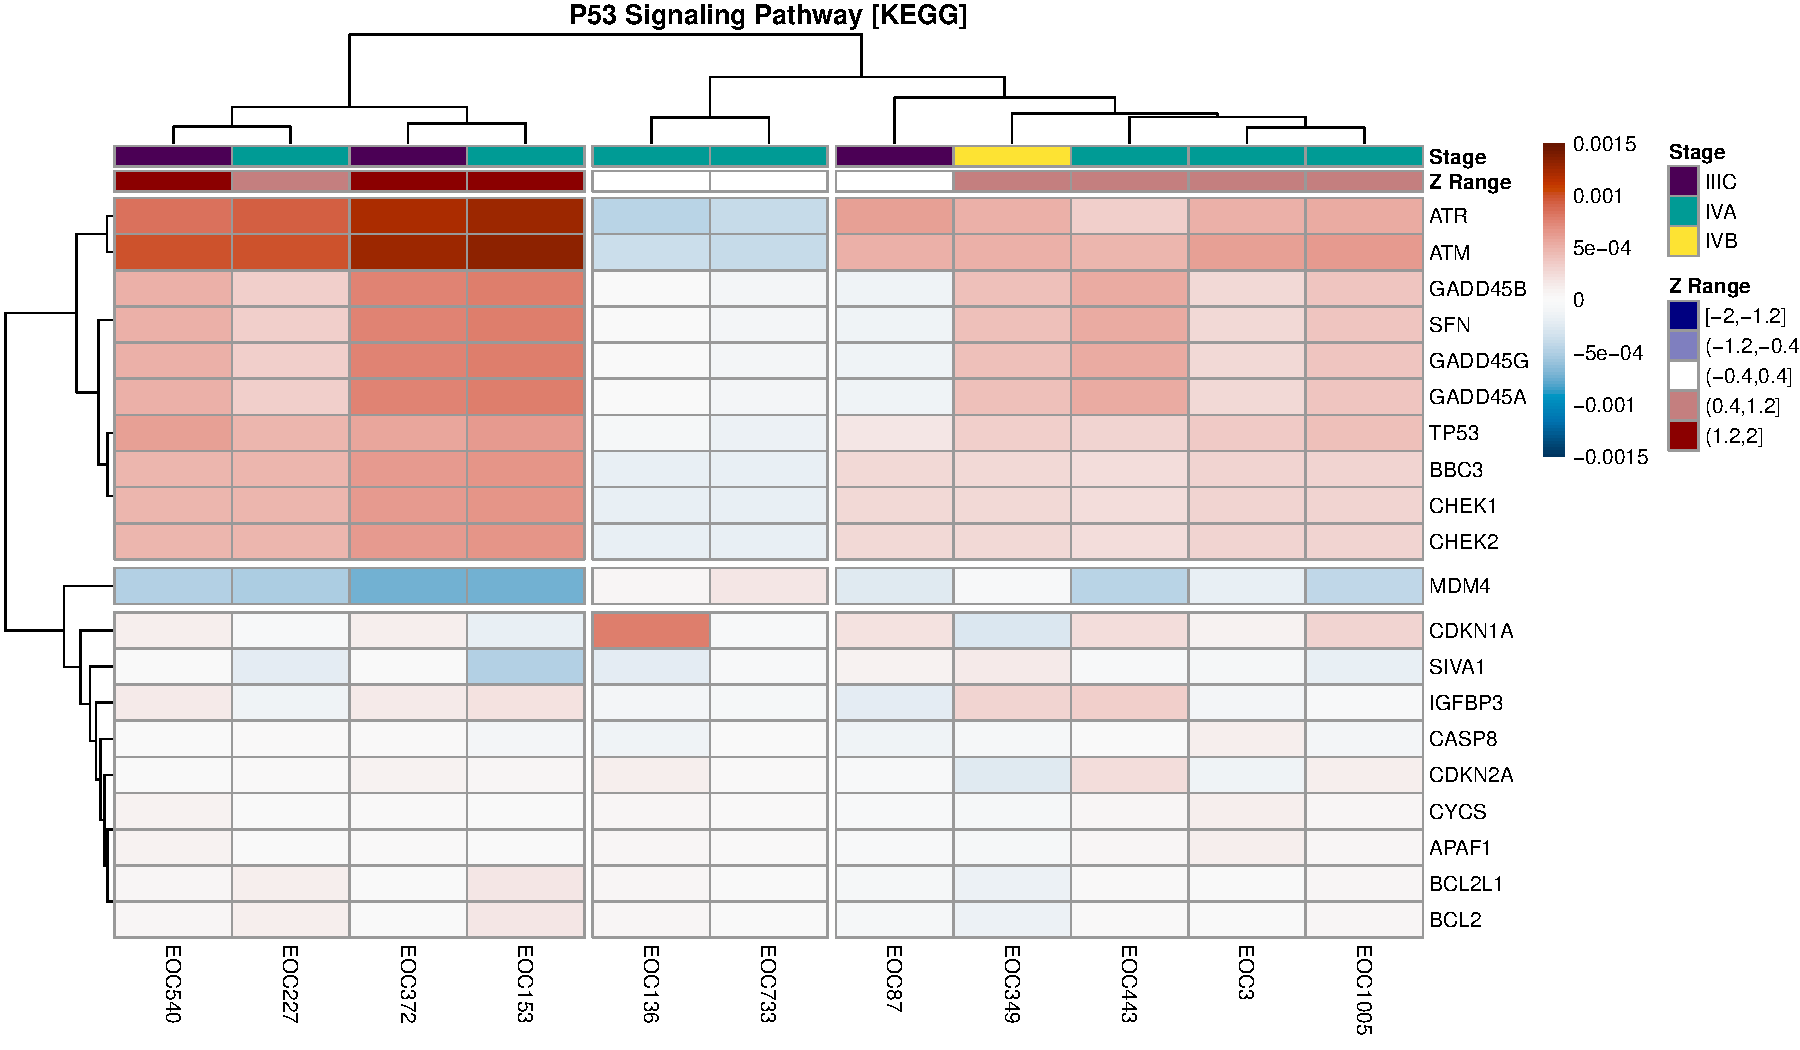
\includegraphics[width=1\linewidth]{sSNAPPY_paper_files/figure-latex/Figure7-1} 

}

\caption{Gene-level perturbation scores for the top 15 genes in the "SUMOylation of DNA replication proteins" pathway ranked by average contribution to the perturbation score. Samples were annotated by patient chemotherapy response score (CRS), along with the range for sample-level Z-scores as a guide to sample-specific pathway perturbation. The genes CDCA8, TOP2A, UBE2I, BIRC5 were identified as possible key drivers of the inhibition of of this pathway.}\label{fig:Figure7}
\end{figure}

From this heatmap we can identify candidate genes which are likely to be making the biggest contribution to the inhibition of the SUMOylation of DNA replication proteins pathway upon chemotherapy,
such as \emph{CDCA8}, \emph{TOP2A}, \emph{UBE2I}, \emph{BIRC5} (Figure \ref{fig:Figure7}).
The four genes are all associated with tumour progression and invasiveness and have been studied in the context of ovarian cancer.
Both ubiquitin conjugating enzyme E2I (\emph{UBE2I}) and cell division cycle associated 8 (\emph{CDCA8}) genes have been identified as oncogenes in numerous cancer types, including ovarian cancer\citep{Dong2013, qi2021}.
Notably, in ovarian cancer, elevated \emph{UBE2I} expression has been associated with poorer clinical outcomes\citep{Zou2020}.
Similarly, expression of \emph{BIRC5} that encodes human survivin protein is also a predictor of inferior ovarian cancer patient outcome\citep{Gasowska-Bajger2021}.
Lastly, Topoisomerase II\(\alpha\) (\emph{TOP2A}), which encodes DNA topoisomerase, has been identified as a gene that promotes the tumorigenesis of HGSOC tumours\citep{Gao2020}.
Aligning with the report by Chekerov et al.\citep{Chekerov2006} that expression of \emph{TOP2A} in ovarian tumour cells decreases as a response to chemotherapy\citep{Chekerov2006}, the median single-sample logFC of \emph{TOP2A} was negative among the HGSOC post-chemotherapy samples included in this study (Figure \ref{fig:Figure8}).
The other three selected potential driver genes (\emph{CDCA8}, \emph{UBE2I}, and \emph{BIRC5}) also had negative median single-sample logFC in post-chemotherapy samples (Figure \ref{fig:Figure8}).
Considering the implication of these four genes in ovarian cancer, decreases in their expression after chemotherapy treatment potentially indicate a favorable response to therapy.
By annotating the heatmap of gene-wise perturbation scores with patient chemotherapy response score (CRS), we noticed that the strongest inhibition of the SUMOylation of DNA replication proteins pathway was in the patient with the highest CRS score of 3 (i.e sample EOC443).
CRS is an indicator of the relative length of progression-free survival after chemotherapy, where a score of 3 represents the longest survival.
Hence inhibition of the SUMOylation of DNA replication proteins pathway might mediate favorable response to chemotherapy in ovarian cancer patients.
We acknowledge that our analysis was limited to a small number of patients, which restricts the generalizability of the results.
However, despite this limitation, these findings underscore the strength of sSNAPPY as a valuable tool for hypothesis generation.
Not only can sSNAPPY predict directional pathway perturbations, but it also enables the identification of key driver genes underlying these perturbations.

\begin{Shaded}
\begin{Highlighting}[]
\NormalTok{gene2plot }\OtherTok{\textless{}{-}}\NormalTok{ entrez2name }\SpecialCharTok{\%\textgreater{}\%}
\NormalTok{    dplyr}\SpecialCharTok{::}\FunctionTok{filter}\NormalTok{(}
\NormalTok{        mapTo }\SpecialCharTok{\%in\%} \FunctionTok{c}\NormalTok{(}\StringTok{"CDCA8"}\NormalTok{, }\StringTok{"TOP2A"}\NormalTok{, }\StringTok{"UBE2I"}\NormalTok{, }\StringTok{"BIRC5"}\NormalTok{)}
\NormalTok{    )}
\NormalTok{(weightedFC}\SpecialCharTok{$}\NormalTok{weighted\_logFC }\SpecialCharTok{/}\NormalTok{ weightedFC}\SpecialCharTok{$}\NormalTok{weight) }\SpecialCharTok{\%\textgreater{}\%}
    \FunctionTok{as.data.frame}\NormalTok{() }\SpecialCharTok{\%\textgreater{}\%}
    \FunctionTok{rownames\_to\_column}\NormalTok{(}\StringTok{"entrezid"}\NormalTok{) }\SpecialCharTok{\%\textgreater{}\%}
    \FunctionTok{pivot\_longer}\NormalTok{(}
        \AttributeTok{cols =} \SpecialCharTok{{-}}\StringTok{"entrezid"}\NormalTok{, }
        \AttributeTok{names\_to =} \StringTok{"sample"}\NormalTok{, }
        \AttributeTok{values\_to =} \StringTok{"ssFC"}
\NormalTok{    ) }\SpecialCharTok{\%\textgreater{}\%}
    \FunctionTok{left\_join}\NormalTok{(entrez2name) }\SpecialCharTok{\%\textgreater{}\%}
\NormalTok{    dplyr}\SpecialCharTok{::}\FunctionTok{filter}\NormalTok{(mapTo }\SpecialCharTok{\%in\%} \FunctionTok{c}\NormalTok{(}\StringTok{"CDCA8"}\NormalTok{, }\StringTok{"TOP2A"}\NormalTok{, }\StringTok{"UBE2I"}\NormalTok{, }\StringTok{"BIRC5"}\NormalTok{)) }\SpecialCharTok{\%\textgreater{}\%}
    \FunctionTok{ggplot}\NormalTok{(}
        \FunctionTok{aes}\NormalTok{(mapTo, ssFC, }\AttributeTok{fill =}\NormalTok{ mapTo)}
\NormalTok{    ) }\SpecialCharTok{+}
    \FunctionTok{geom\_boxplot}\NormalTok{() }\SpecialCharTok{+}
    \FunctionTok{labs}\NormalTok{(}
        \AttributeTok{x =} \StringTok{""}\NormalTok{, }
        \AttributeTok{fill =} \StringTok{"Gene"}
\NormalTok{    ) }\SpecialCharTok{+}
    \FunctionTok{geom\_hline}\NormalTok{(}\AttributeTok{yintercept =} \DecValTok{0}\NormalTok{, }\AttributeTok{color =} \StringTok{"red"}\NormalTok{, }\AttributeTok{linetype =} \StringTok{"dashed"}\NormalTok{) }\SpecialCharTok{+}
    \FunctionTok{theme\_bw}\NormalTok{() }\SpecialCharTok{+}
    \FunctionTok{theme}\NormalTok{(}
        \AttributeTok{text =} \FunctionTok{element\_text}\NormalTok{(}\AttributeTok{size =} \DecValTok{10}\NormalTok{)}
\NormalTok{    )}
\end{Highlighting}
\end{Shaded}

\begin{figure}

{\centering 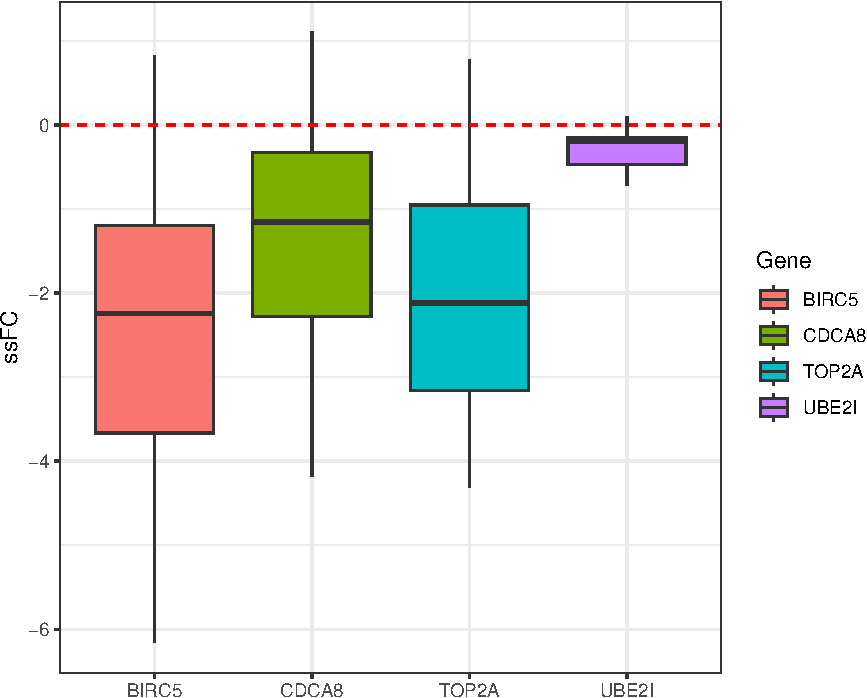
\includegraphics[width=0.8\linewidth]{sSNAPPY_paper_files/figure-latex/Figure8-1} 

}

\caption{Single-sample logFC (ssFC) of potential key genes driving the inhibition of "SUMOylation of DNA replication proteins" pathway as a response to chemotherapy in HGSOC tumours.}\label{fig:Figure8}
\end{figure}

\hypertarget{discussion}{%
\section{Discussion}\label{discussion}}

In conclusion, we have presented and provided a demonstration for the R/Bioconductor package \emph{sSNAPPY} which offers a novel single-sample pathway perturbation testing approach, tailored for heterogeneous tissue samples in matched-pair design.
In contrast to many common enrichment methods, sSNAPPY uses pathway topology information to compute perturbation scores which indicate the likely impact on the activity of a pathway, by predicting direction of change and enabling deeper characterisation of biological responses.
By applying sSNAPPY to a public scRNA-seq data collected before and after HGSOC patients were subjected to chemotherapy, we demonstrated its ability to detect significant pathway perturbations of various interesting biological processes consistent with, and far beyond what was shown in the original study.
Whilst initially conceived for bulk-RNA studies, this demonstration has also provided clear applicability to scRNA datasets.
\emph{sSNAPPY} addresses the limitations of alternative strategies which fail to account for gene-gene interactions encoded by pathway topologies and are unable to predict the directionality of pathway activities.
In addition, the single-sample nature of the method can be utilised to address the increasing demand for personalised medicine.
Through identifying shared and divergent responses between individuals, \emph{sSNAPPY} can provide valuable insights into the heterogeneous responses across clinical samples.
Overall, we believe sSNAPPY represents a valuable addition to the existing body of pathway analysis methods.

\hypertarget{data-availability}{%
\section{Data availability}\label{data-availability}}

The dataset analysed in this manuscript are stored in the data directory of this GitHub repository.

\hypertarget{software-availability}{%
\section{Software availability}\label{software-availability}}

\begin{itemize}
\item
  Software available from: \url{https://bioconductor.org/packages/release/bioc/html/sSNAPPY.html}
\item
  Source code available from: \url{https://github.com/Wenjun-Liu/sSNAPPY}
\item
  Archived source code at time of publication: \url{https://doi.org/10.5281/zenodo.8185451}
\item
  License: GNU General Public License v3.0 (\href{https://opensource.org/license/gpl-3-0/}{GPL-3}
\end{itemize}

\hypertarget{author-contributions}{%
\section{Author Contributions}\label{author-contributions}}

WL's contributions include Conceptualization, Data Curation, Formal Analysis, Investigation, Methodology, Project Administration, Software, Validation, Visualisation, Writing - Original Draft Preparation, and Writing - Review \& Editing.
VM was involved with Conceptualization, Methodology and Writing - Review \& Editing.
WDT contributed to Writing - Review \& Editing.
SMP's contributions include Conceptualization, Methodology, Project Administration, Software, Supervision, Writing - Original Draft Preparation, and Writing - Review \& Editing.

\hypertarget{competing-interests}{%
\section{Competing interests}\label{competing-interests}}

No competing interests were disclosed

\hypertarget{grant-information}{%
\section{Grant information}\label{grant-information}}

W.D. Tilley's research is supported by the National Health and Medical Research Council of Australia (ID 1186647) and the National Breast Cancer Foundation Australia (ID IIRS-23-069)

\renewcommand\refname{References}
{\small\bibliography{bibliography.bib}}

\end{document}
